% Options for packages loaded elsewhere
% Options for packages loaded elsewhere
\PassOptionsToPackage{unicode}{hyperref}
\PassOptionsToPackage{hyphens}{url}
\PassOptionsToPackage{dvipsnames,svgnames,x11names}{xcolor}
%
\documentclass[
  11pt,
  11pt,
  letterpaper]{article}
\usepackage{xcolor}
\usepackage[margin=1in,top=1.25in,bottom=1.25in]{geometry}
\usepackage{amsmath,amssymb}
\setcounter{secnumdepth}{5}
\usepackage{iftex}
\ifPDFTeX
  \usepackage[T1]{fontenc}
  \usepackage[utf8]{inputenc}
  \usepackage{textcomp} % provide euro and other symbols
\else % if luatex or xetex
  \usepackage{unicode-math} % this also loads fontspec
  \defaultfontfeatures{Scale=MatchLowercase}
  \defaultfontfeatures[\rmfamily]{Ligatures=TeX,Scale=1}
\fi
\usepackage{lmodern}
\ifPDFTeX\else
  % xetex/luatex font selection
\fi
% Use upquote if available, for straight quotes in verbatim environments
\IfFileExists{upquote.sty}{\usepackage{upquote}}{}
\IfFileExists{microtype.sty}{% use microtype if available
  \usepackage[]{microtype}
  \UseMicrotypeSet[protrusion]{basicmath} % disable protrusion for tt fonts
}{}
\usepackage{setspace}
\makeatletter
\@ifundefined{KOMAClassName}{% if non-KOMA class
  \IfFileExists{parskip.sty}{%
    \usepackage{parskip}
  }{% else
    \setlength{\parindent}{0pt}
    \setlength{\parskip}{6pt plus 2pt minus 1pt}}
}{% if KOMA class
  \KOMAoptions{parskip=half}}
\makeatother
% Make \paragraph and \subparagraph free-standing
\makeatletter
\ifx\paragraph\undefined\else
  \let\oldparagraph\paragraph
  \renewcommand{\paragraph}{
    \@ifstar
      \xxxParagraphStar
      \xxxParagraphNoStar
  }
  \newcommand{\xxxParagraphStar}[1]{\oldparagraph*{#1}\mbox{}}
  \newcommand{\xxxParagraphNoStar}[1]{\oldparagraph{#1}\mbox{}}
\fi
\ifx\subparagraph\undefined\else
  \let\oldsubparagraph\subparagraph
  \renewcommand{\subparagraph}{
    \@ifstar
      \xxxSubParagraphStar
      \xxxSubParagraphNoStar
  }
  \newcommand{\xxxSubParagraphStar}[1]{\oldsubparagraph*{#1}\mbox{}}
  \newcommand{\xxxSubParagraphNoStar}[1]{\oldsubparagraph{#1}\mbox{}}
\fi
\makeatother


\usepackage{longtable,booktabs,array}
\usepackage{calc} % for calculating minipage widths
% Correct order of tables after \paragraph or \subparagraph
\usepackage{etoolbox}
\makeatletter
\patchcmd\longtable{\par}{\if@noskipsec\mbox{}\fi\par}{}{}
\makeatother
% Allow footnotes in longtable head/foot
\IfFileExists{footnotehyper.sty}{\usepackage{footnotehyper}}{\usepackage{footnote}}
\makesavenoteenv{longtable}
\usepackage{graphicx}
\makeatletter
\newsavebox\pandoc@box
\newcommand*\pandocbounded[1]{% scales image to fit in text height/width
  \sbox\pandoc@box{#1}%
  \Gscale@div\@tempa{\textheight}{\dimexpr\ht\pandoc@box+\dp\pandoc@box\relax}%
  \Gscale@div\@tempb{\linewidth}{\wd\pandoc@box}%
  \ifdim\@tempb\p@<\@tempa\p@\let\@tempa\@tempb\fi% select the smaller of both
  \ifdim\@tempa\p@<\p@\scalebox{\@tempa}{\usebox\pandoc@box}%
  \else\usebox{\pandoc@box}%
  \fi%
}
% Set default figure placement to htbp
\def\fps@figure{htbp}
\makeatother


% definitions for citeproc citations
\NewDocumentCommand\citeproctext{}{}
\NewDocumentCommand\citeproc{mm}{%
  \begingroup\def\citeproctext{#2}\cite{#1}\endgroup}
\makeatletter
 % allow citations to break across lines
 \let\@cite@ofmt\@firstofone
 % avoid brackets around text for \cite:
 \def\@biblabel#1{}
 \def\@cite#1#2{{#1\if@tempswa , #2\fi}}
\makeatother
\newlength{\cslhangindent}
\setlength{\cslhangindent}{1.5em}
\newlength{\csllabelwidth}
\setlength{\csllabelwidth}{3em}
\newenvironment{CSLReferences}[2] % #1 hanging-indent, #2 entry-spacing
 {\begin{list}{}{%
  \setlength{\itemindent}{0pt}
  \setlength{\leftmargin}{0pt}
  \setlength{\parsep}{0pt}
  % turn on hanging indent if param 1 is 1
  \ifodd #1
   \setlength{\leftmargin}{\cslhangindent}
   \setlength{\itemindent}{-1\cslhangindent}
  \fi
  % set entry spacing
  \setlength{\itemsep}{#2\baselineskip}}}
 {\end{list}}
\usepackage{calc}
\newcommand{\CSLBlock}[1]{\hfill\break\parbox[t]{\linewidth}{\strut\ignorespaces#1\strut}}
\newcommand{\CSLLeftMargin}[1]{\parbox[t]{\csllabelwidth}{\strut#1\strut}}
\newcommand{\CSLRightInline}[1]{\parbox[t]{\linewidth - \csllabelwidth}{\strut#1\strut}}
\newcommand{\CSLIndent}[1]{\hspace{\cslhangindent}#1}



\setlength{\emergencystretch}{3em} % prevent overfull lines

\providecommand{\tightlist}{%
  \setlength{\itemsep}{0pt}\setlength{\parskip}{0pt}}



 


% ArXiv-style preamble for proper author metadata display
% Improve PDF text extraction: disable ligatures that cause copy-paste artifacts
\usepackage{microtype}
\usepackage{hyperref}
\hypersetup{
    colorlinks=true,
    linkcolor=blue,
    citecolor=blue,
    urlcolor=blue,
    pdfauthor={Mohammad Dastgheib and Fatemeh Pourmahdian},
    pdftitle={Adaptive Gaze-Hand Switching in XR: Modality-Specific Failure Modes and the Midas Touch Problem},
    pdfkeywords={Extended Reality, Virtual Reality, Adaptive Interfaces, Gaze Interaction, Fitts's Law, Human-Computer Interaction, Multimodal Interaction, Pupillometry}
}

% Required packages
\usepackage{amsmath}
\usepackage{amssymb}
\usepackage{graphicx}
\usepackage{booktabs}
\usepackage{orcidlink}
\usepackage{float}

% Force figures and tables to appear exactly where placed (no floating)
\floatplacement{figure}{H}
\floatplacement{table}{H}

% Keep tables from splitting awkwardly: require space before each table
\usepackage{needspace}
\usepackage{etoolbox}
\BeforeBeginEnvironment{table}{\Needspace{10\baselineskip}}

% Customize title page formatting with proper author block
\makeatletter
\renewcommand{\@maketitle}{%
  \newpage
  \null
  \vskip 2em%
  \begin{center}%
    \let \footnote \thanks
    {\LARGE \@title \par}%
    \vskip 1.5em%
    {\large
      \begin{tabular}[t]{c}%
        Mohammad Dastgheib\textsuperscript{1} \orcidlink{0000-0001-7684-3731} \\
        University of California, Riverside \\
        \href{mailto:mohammad.dastgheib@email.ucr.edu}{\texttt{mohammad.dastgheib@email.ucr.edu}} \\[0.5em]
        Fatemeh Pourmahdian \orcidlink{0009-0007-5473-2070} \\
        \href{mailto:fatemepourmahd@gmail.com}{\texttt{fatemepourmahd@gmail.com}}
      \end{tabular}\par}%
    \vskip 1em%
    {\large \@date \par}%
  \end{center}%
  \vskip 0.5em%
  \begin{center}
    \footnotesize
    \begin{tabular}{@{}l@{}}
      \textsuperscript{1}Corresponding author: \href{mailto:mohammad.dastgheib@email.ucr.edu}{\texttt{mohammad.dastgheib@email.ucr.edu}}
    \end{tabular}
  \end{center}%
  \par
  \vskip 1.5em%
}
\makeatother
\makeatletter
\@ifpackageloaded{caption}{}{\usepackage{caption}}
\AtBeginDocument{%
\ifdefined\contentsname
  \renewcommand*\contentsname{Table of contents}
\else
  \newcommand\contentsname{Table of contents}
\fi
\ifdefined\listfigurename
  \renewcommand*\listfigurename{List of Figures}
\else
  \newcommand\listfigurename{List of Figures}
\fi
\ifdefined\listtablename
  \renewcommand*\listtablename{List of Tables}
\else
  \newcommand\listtablename{List of Tables}
\fi
\ifdefined\figurename
  \renewcommand*\figurename{Figure}
\else
  \newcommand\figurename{Figure}
\fi
\ifdefined\tablename
  \renewcommand*\tablename{Table}
\else
  \newcommand\tablename{Table}
\fi
}
\@ifpackageloaded{float}{}{\usepackage{float}}
\floatstyle{ruled}
\@ifundefined{c@chapter}{\newfloat{codelisting}{h}{lop}}{\newfloat{codelisting}{h}{lop}[chapter]}
\floatname{codelisting}{Listing}
\newcommand*\listoflistings{\listof{codelisting}{List of Listings}}
\makeatother
\makeatletter
\makeatother
\makeatletter
\@ifpackageloaded{caption}{}{\usepackage{caption}}
\@ifpackageloaded{subcaption}{}{\usepackage{subcaption}}
\makeatother
\usepackage{bookmark}
\IfFileExists{xurl.sty}{\usepackage{xurl}}{} % add URL line breaks if available
\urlstyle{same}
\hypersetup{
  pdftitle={Adaptive Gaze-Hand Switching in XR: Modality-Specific Failure Modes and the Midas Touch Problem},
  pdfauthor={Mohammad Dastgheib; Fatemeh Pourmahdian},
  colorlinks=true,
  linkcolor={blue},
  filecolor={Maroon},
  citecolor={blue},
  urlcolor={blue},
  pdfcreator={LaTeX via pandoc}}


\title{Adaptive Gaze-Hand Switching in XR: Modality-Specific Failure
Modes and the Midas Touch Problem}
\author{Mohammad Dastgheib \and Fatemeh Pourmahdian}
\date{2026-03-06}
\begin{document}
\maketitle
\begin{abstract}
Extended Reality (XR) interfaces impose both ergonomic and cognitive
demands, yet current systems often force a binary choice between
hand-based input, which can produce fatigue, and gaze-based input, which
is vulnerable to the Midas Touch problem and precision limitations. We
introduce the xr-adaptive-modality-2025 platform, a web-based
open-source framework for studying whether context-driven adaptive
switching between gaze and hand input can improve XR pointing
performance and reduce workload relative to static unimodal interaction.
The platform combines physiologically accurate gaze simulation, an ISO
9241-9 multidirectional tapping task, and two modality-specific adaptive
interventions: gaze declutter and hand target-width inflation. We
evaluated the system in a 2 × 2 × 2 within-subjects design manipulating
Modality (Hand vs.~Gaze), UI Mode (Static vs.~Adaptive), and Pressure
(Yes vs.~No). Interim results from N=23 participants show that hand
yielded higher throughput than gaze (5.15 vs.~4.70 bits/s), lower error
(1.75\% vs.~18.65\%), and lower NASA-TLX workload. Crucially, error
profiles differed sharply by modality: gaze errors were predominantly
slips (99.2\%), whereas hand errors were predominantly misses (95.7\%),
strongly supporting the Midas Touch account. Of the two adaptive
interventions, only gaze declutter executed in this dataset; it modestly
reduced timeouts but not slips. Hand width inflation was not evaluable
due to a UI integration bug. These findings reveal modality-specific
failure modes with direct implications for adaptive policy design, and
establish the platform as a reproducible infrastructure for confirmatory
studies. Full confirmatory analyses will be reported at the planned
complete sample of N=48.
\end{abstract}


\setstretch{1}
\vspace{-0.5em}

\textbf{Keywords:} Extended Reality, Adaptive Interfaces, Gaze
Interaction, Fitts's Law, Multimodal Interaction, Gaze Simulation, Midas
Touch, Linear Ballistic Accumulator, Intent Disambiguation

\newpage

\section{Introduction}\label{introduction}

XR interaction changes the control demands of pointing by moving input
from desktop devices to embodied hand and gaze actions. Unlike the
desktop metaphor, where interaction is mediated by low-effort devices
like the mouse and keyboard, XR requires the user to engage their entire
body; the primary pointing devices are the user's own hands and eyes.
This embodied interaction is fraught with ergonomic and cognitive
challenges. The ``Gorilla Arm'' syndrome, a phenomenon where prolonged
mid-air arm extension leads to rapid musculoskeletal fatigue and pain,
remains a critical barrier to the long-term adoption of gestural
interfaces. Conversely, gaze-based interaction, which leverages the
speed of the human oculomotor system, suffers from the ``Midas Touch''
problem---the inherent ambiguity between looking for perception and
looking for action---and lacks the fine motor precision required for
granular manipulation tasks (Jacob, 1990).

Current XR systems typically force a binary choice: the user must either
commit to a controller-based paradigm, accepting the physical fatigue,
or a gaze-based paradigm, accepting the lack of precision and the
potential for inadvertent triggers. This rigid dichotomy ignores the
dynamic nature of human attention and the varying demands of different
tasks. A high-precision manipulation task may require the stability of a
hand controller, while a rapid visual search task is best served by the
saccadic speed of the eye.

We introduce the xr-adaptive-modality-2025 platform, a research
framework for studying adaptive switching between hand and gaze input in
XR. The system combines an ISO 9241-9 pointing task, physiologically
informed gaze simulation, and modality-specific adaptive interventions
intended to address distraction during gaze selection and spatial
difficulty during hand selection. The central question is whether
adaptive modality logic can improve performance and workload relative to
static unimodal interaction (Soukoreff \& MacKenzie, 2004).

This paper makes three contributions. First, we present an
\textbf{open-source platform} for controlled, reproducible study of
adaptive gaze--hand switching in XR, including a physiologically
informed gaze simulation, a policy-driven adaptation engine, and a full
remote data collection infrastructure. Second, we provide
\textbf{quantitative empirical evidence} on gaze vs.~hand input in an
ISO 9241-9 pointing task (N=23 interim), showing that hand substantially
outperforms gaze on throughput (5.15 vs.~4.70 bits/s) and error rate
(1.75\% vs.~18.65\%), and that the dominant failure modes are
modality-specific: slips (false activations) for gaze and misses
(spatial targeting failures) for hand. Third, we demonstrate that a
simple \textbf{gaze-declutter adaptation} modestly reduces timeouts but
does not address the core slip-based failure mode of gaze interaction,
which has direct implications for designing adaptive modality policies.
Unlike prior gaze+hand paradigms that treat the two modalities as
complementary components of a fixed multimodal combination (e.g., gaze
for acquisition + hand for confirmation (Jacob, 1990)), this work
investigates \emph{context-driven switching}---when and how the system
should shift between modalities based on real-time performance signals.

\section{Background and Related Work}\label{background-and-related-work}

\subsection{The Sensorimotor Implications of Spatial
Input}\label{the-sensorimotor-implications-of-spatial-input}

To design an effective adaptive system, one must first deconstruct the
physiological mechanisms of the component modalities. Hand and gaze
afford different control properties in XR: hand input supports precise
corrective control, whereas gaze supports rapid orienting but introduces
ambiguity when fixation is used for selection.

\textbf{Manual Pointing in XR:} Manual input in XR, whether through held
controllers or optical hand tracking, mimics the act of physical
pointing. This interaction style benefits from proprioception---the
body's innate sense of limb position---which allows for high-precision
corrections without visual attention. However, the biomechanical cost is
substantial. In a 1:1 mapped XR environment, reaching a virtual object
requires a corresponding physical motion. Frequent large-amplitude
movements lead to fatigue in the deltoids and trapezius muscles. As
fatigue sets in, the signal-to-noise ratio of the motor system degrades;
the hand begins to tremor, increasing the effective target width
required for accurate selection and reducing the overall throughput of
the interaction.

\textbf{Gaze Interaction:} The eye is the fastest motor organ in the
human body. Saccades---rapid, ballistic movements of the eye---can reach
velocities exceeding 900 degrees per second (Bahill \& Stark, 1979),
making gaze an incredibly efficient modality for target acquisition.
However, the eye is fundamentally an input organ, not an output device.
Using gaze for selection introduces several critical issues: (1)
\textbf{The Midas Touch}---in the physical world, we can look at an
object without interacting with it, but in a gaze-controlled interface,
looking becomes equivalent to touching, requiring ``dwell time''
mechanisms that slow interaction (Jacob, 1990); (2)
\textbf{Microsaccades and Jitter}---even when ``fixated,'' the eye
performs microsaccades to refresh the retinal image (Martinez-Conde et
al., 2004), meaning a gaze cursor is inherently noisy, making selection
of small targets frustrating without smoothing algorithms; (3)
\textbf{Saccadic Suppression}---during rapid eye movements, the visual
system suppresses input to prevent motion blur (Bridgeman et al., 1975),
creating a ``blind'' phase that makes the initial phase of gaze
targeting effectively open-loop.

\subsection{Signal Processing and Cognitive Load
Theory}\label{signal-processing-and-cognitive-load-theory}

To study these dynamics controllably, our platform employs a generative
simulation rather than raw sensor input. This simulation introduces
three key constraints derived from oculomotor physiology: (1)
\textbf{Sensor Lag}---a first-order lag (linear interpolation) mimics
the processing latency (30--70 ms) typical of video-based eye trackers
(Saunders \& Woods, 2014); (2) \textbf{Saccadic Blindness}---the cursor
is frozen during high-velocity movements (\textgreater120 deg/s),
simulating the lack of visual feedback during a saccade (Bridgeman et
al., 1975); (3) \textbf{Fixation Jitter}---Gaussian noise is injected at
low velocities to mimic fixational drift and tremor (Martinez-Conde et
al., 2004), ensuring that the ``cost'' of gaze interaction is accurately
represented even when using a mouse proxy.

We use Cognitive Load Theory (CLT) as a conceptual lens for reasoning
about modality-specific costs (Sweller, 1988). CLT distinguishes
intrinsic load (task difficulty) from extraneous load (interface
overhead). In principle, hand input may increase physical effort
(intrinsic load during larger reaches), whereas gaze input may increase
extraneous attentional and verification demands during precise
selection. The present study uses workload (NASA-TLX) and performance
measures to test whether these modality-specific costs appear in the
current task, and whether adaptive interventions can reduce them.

\subsection{Adaptive Intervention
Mechanisms}\label{adaptive-intervention-mechanisms}

We implemented two modality-specific adaptive interventions. \textbf{For
gaze interaction}, a declutter mechanism draws on visual attention
guiding techniques in XR, related to diminished reality (DR) (Herling \&
Broll, 2010). When the policy engine detects performance degradation in
gaze mode (error burst or RT threshold exceeded), non-critical HUD
elements are hidden, mitigating peripheral distraction. This aligns with
foveated rendering principles, where systems leverage the human visual
system's foveal focus to prioritize content (Patney et al., 2016). By
decluttering when performance degrades, we hypothesize that gaze-based
targeting becomes faster and less cognitively demanding.

\textbf{For hand-based interactions}, our adaptive strategy is width
inflation---dynamically expanding the effective size of targets when
performance degrades, triggered by the policy engine based on error rate
and reaction time thresholds. This concept is inspired by ``expanding
targets'' research (McGuffin \& Balakrishnan, 2005) and the ``Bubble
Cursor'' (Grossman \& Balakrishnan, 2005), which demonstrate that even
slight enlargement significantly improves pointing performance. Our
implementation uses a hysteresis gate (requiring N consecutive trials
meeting trigger conditions) to prevent flicker, acting as a ``safety
net'' that compensates for motor tremor under fatigue. In the current
interim dataset, the hand width-inflation pathway was not evaluable:
width scaling remained at 1.0 across trials, and although the policy
engine emitted inflate-width actions in some sessions, the rendered
targets were not updated.

\textbf{Differentiation from prior gaze+hand work.} Recent XR systems
combine gaze and hand in fixed multimodal combinations: gaze for target
acquisition and hand for confirmation or manipulation (Pfeuffer et al.,
2017, 2024). Pfeuffer et al. (Pfeuffer et al., 2024) outline design
principles for gaze+pinch interaction (e.g., division of labor,
minimalistic timing), while Kim et al. (Kim et al., 2025) propose
PinchCatcher, a semi-pinch quasi-mode for multi-selection in gaze+pinch
interfaces. These approaches treat gaze and hand as complementary
components of a fixed interaction paradigm. Our work differs by
investigating \emph{context-driven switching}---when and how the system
should shift between modalities based on real-time performance
signals---rather than a fixed multimodal combination. We draw on
context-aware computing principles (Dey, 2001) to frame policy-driven
adaptation that responds to performance degradation.

\section{Research Objectives}\label{research-objectives}

The primary objective of this research is to validate the efficacy of
the \texttt{xr-adaptive-modality-2025} platform. The study is guided by
three core research questions:

\textbf{RQ1 (Performance):} Does a context-aware adaptive system yield
higher throughput (\(TP\)) than static unimodal systems?

\textbf{RQ2 (Workload):} Can adaptive modality switching reduce
``Physical Demand'' and ``Frustration'' (NASA-TLX) compared to
traditional interaction?

\textbf{RQ3 (Adaptation):} Do adaptive interventions (declutter, width
inflation) improve performance and reduce workload relative to
non-adaptive conditions?

\section{Theoretical Framework}\label{theoretical-framework}

This section establishes the mathematical and psychological models that
underpin the system's logic, specifically focusing on Information Theory
as applied to human movement and the neuroergonomics of attention.

\subsection{Fitts's Law: The Information Capacity of the Human Motor
System}\label{fittss-law-the-information-capacity-of-the-human-motor-system}

Fitts's Law (1954) is robustly established as the governing dynamic of
pointing tasks. It frames movement not as a physical event, but as an
information transmission task. The ``difficulty'' of a target is
measured in bits, representing the amount of information the motor
system must process to resolve the movement successfully. We adopt the
\textbf{Shannon Formulation}, the standard for ISO 9241-9 compliance, as
it better models the information entropy of the task and avoids negative
ID values for very close targets:

\[ID = \log_2 \left( \frac{D}{W} + 1 \right)\]

Movement Time (\(MT\)) is then modeled as a linear function of this
difficulty:

\[MT = a + b \cdot ID\]

Where the intercept \(a\) represents non-informational additive
components (e.g., reaction time, system latency) and the slope \(b\)
represents the rate of information processing. The reciprocal of the
slope, \(1/b\), is often referred to as the \textbf{Index of
Performance} (\(IP\)), or bandwidth, measured in bits per second.

\subsection{The Speed-Accuracy Tradeoff in
3D}\label{the-speed-accuracy-tradeoff-in-3d}

In XR, the ``Width'' (\(W\)) of a target is ambiguous. To standardize
performance across users with varying error rates, the
\texttt{xr-adaptive-modality-2025} platform utilizes the
\textbf{Effective Width} (\(W_e\)). Unlike nominal width, \(W_e\) is
derived from the spatial distribution of selection endpoints.

Consistent with ISO 9241-9, we calculate \(W_e\) using the standard
deviation of selection coordinates projected onto the task axis. For a
target at position \(P_{target}\) and a starting position \(P_{start}\),
the task axis vector is \(\vec{v} = P_{target} - P_{start}\). The
projected error \(x_i\) for a trial \(i\) with endpoint \(P_{hit}\) is
computed as the scalar projection:

\[x_i = \frac{(P_{hit} - P_{target}) \cdot \vec{v}}{\| \vec{v} \|}\]

The effective width is then calculated as \(W_e = 4.133 × \sigma_x\),
where \(\sigma_x\) is the standard deviation of these projected errors.
This effectively normalizes the error rate to 4\%, allowing us to
calculate \textbf{Throughput} (\(TP\)), a unified metric of speed and
accuracy:

\[TP = \frac{ID_e}{MT} = \frac{\log_2(D/W_e + 1)}{MT}\]

This metric is critical for comparing Modality A (Gaze) vs.~Modality B
(Hand). Gaze might have a lower \(MT\) due to saccadic speed, but if its
jitter results in a massive \(W_e\) (low accuracy), the overall
Throughput will be lower.

\subsection{Modeling Movement and Decision
Processes}\label{modeling-movement-and-decision-processes}

To decompose the underlying processes of movement execution and decision
verification, we employ a \textbf{Hybrid Analysis Framework} that
separates the ballistic trajectory from the final selection decision.

\subsubsection{Control Theory and Submovement
Models}\label{control-theory-and-submovement-models}

The \textbf{Optimized Submovement Model} (Meyer et al., 1988) posits
that pointing movements are composed of a primary ballistic impulse
followed by \(n\) corrective submovements. The total movement time is
the sum of the primary movement duration and the duration of subsequent
corrections required to bring the endpoint error within the target
bounds.

We quantify the ``cost of control'' by analyzing the velocity profile
\(v(t)\) of the cursor. A submovement is mathematically identified as a
zero-crossing in the acceleration profile (or a local maximum in
velocity) after the initial ballistic phase. The \textbf{Submovement
Count} (\(N_{sub}\)) serves as a proxy for the efficiency of the control
loop:

\[N_{sub} = \sum_{t=0}^{T} \mathbb{1}(\text{is\_velocity\_peak}(t)) - 1\]

In gaze-based interaction, simulated lag and saccadic blindness force
users into an intermittent control regime, theoretically increasing
\(N_{sub}\). Submovement and path-quality analyses are part of the
broader pipeline and will be reported in the full confirmatory sample.

\subsubsection{The Linear Ballistic Accumulator (LBA)
Model}\label{the-linear-ballistic-accumulator-lba-model}

Once the cursor enters the target, users face a decision verification
problem: ``Is the cursor stable enough to click?'' We model this using
the \textbf{Linear Ballistic Accumulator (LBA)} (Brown \& Heathcote,
2008). LBA treats the decision as a race between independent
accumulators (e.g., ``Select'' vs.~``Wait/Drift'').

For the \(i\)-th accumulator, evidence \(x_i(t)\) accumulates linearly
over time \(t\) from a starting point \(A\) with a drift rate \(d_i\):

\[x_i(t) = A + d_i \cdot t\]

The starting point \(A\) is drawn from a uniform distribution
\(U[0, A_{max}]\), and the drift rate \(d_i\) is drawn from a normal
distribution \(N(v_i, s)\). A decision is made when the evidence reaches
a threshold \(b\).

Unlike Drift Diffusion Models (DDM) which require substantial error
rates to constrain the boundary separation (Lerche et al., 2017), LBA is
robust to the low-error scenarios typical of Fitts' tasks. It allows us
to explicitly estimate the \textbf{Caution Threshold} (\(b - A\))---the
amount of evidence users require before committing to selection. We
hypothesize that adaptive interventions can alter the amount of evidence
users require before committing to selection.

\section{Methods}\label{methods}

The study was designed to support reproducible evaluation of adaptive
modality switching under controlled remote testing conditions. The
platform \texttt{xr-adaptive-modality-2025} serves as the technical
apparatus for the study.

\subsection{Apparatus and
Participants}\label{apparatus-and-participants}

We developed a custom pointing testbed as a web-based application (React
18, TypeScript), allowing broad hardware compatibility for remote
participants. The study was conducted on participants' own computers
using a standard mouse or trackpad.

\subsubsection{Display Calibration and Reliability
Measures}\label{display-calibration-and-reliability-measures}

To ensure measurement validity across heterogeneous display
configurations, we implemented a multi-layered approach addressing
display variability. Before commencing experimental trials, participants
completed a \textbf{Credit Card Calibration} procedure: participants
placed a standard credit card (85.60 mm × 53.98 mm) on their screen and
adjusted an on-screen rectangle to match its physical dimensions. This
calibration enabled computation of pixels per millimeter (px/mm) and
pixels per degree of visual angle (PPD), normalizing gaze simulation
jitter to screen-space pixels and ensuring consistent perceptual
difficulty across different display sizes and resolutions (MacKenzie,
1992).

To minimize measurement error, we enforced strict display requirements:
fullscreen/maximized window (required before starting blocks), browser
zoom locked to 100\% (verified before each block using
\texttt{window.visualViewport.scale}), and live monitoring during trials
(trials automatically paused if settings changed). For every trial, we
logged comprehensive display metadata: device pixel ratio (DPR), browser
type, viewport dimensions, zoom level, fullscreen status, and tab
visibility duration. Trials were excluded from analysis if zoom level ≠
100\%, fullscreen status = FALSE, DPR instability (change \textgreater{}
0.1 between blocks), or tab hidden for \textgreater{} 500ms.
Participants with \textgreater40\% of trials excluded due to display
violations were removed from the final analysis.

\subsubsection{Gaze Simulation (The ``Ground Truth''
Signal)}\label{gaze-simulation-the-ground-truth-signal}

To ensure rigorous internal validity and precise control over noise
characteristics, we utilized a \textbf{Physiologically-Accurate Gaze
Simulation}. This approach allowed us to model the specific constraints
of eye-tracking interaction---latency and jitter---with precise control
over noise characteristics. The simulation transformed raw mouse input
into ``gaze'' coordinates via three mechanisms derived from oculomotor
physiology:

\begin{enumerate}
\def\labelenumi{\arabic{enumi}.}
\item
  \textbf{Saccadic Suppression \& Ballistic Movement:} The cursor was
  ``frozen'' (blind) during high-velocity movements (\textgreater120
  deg/s) to simulate the brain's suppression of visual input during
  saccades, a phenomenon known as saccadic suppression of image
  displacement (Bridgeman et al., 1975). This aligns with the ballistic
  nature of saccadic eye movements, where visual feedback is effectively
  open-loop until the eye settles.
\item
  \textbf{Fixation Jitter \& Drift:} When the cursor slowed (\textless30
  deg/s), Gaussian noise (SD \(\approx\) 0.12\(^\circ\) visual angle)
  was injected to simulate fixational eye movements (Martinez-Conde et
  al., 2004), specifically the random walk characteristics of ocular
  drift and tremor that occur even during attempted fixation. This
  angular noise was normalized to screen pixels using the
  pixels-per-degree (PPD) calibration value, ensuring consistent
  perceptual difficulty across different display sizes and viewing
  distances.
\item
  \textbf{Sensor Lag:} A first-order lag (linear interpolation, factor
  0.15) was applied to mimic the processing latency (typically 30--70
  ms) inherent in video-based eye trackers (Saunders \& Woods, 2014).
\end{enumerate}

\subsection{Input Modality
Implementations}\label{input-modality-implementations}

The system implemented two distinct input modalities, each with static
and adaptive modes. \textbf{For hand-based trials}, participants
controlled a cursor with their mouse to click the target. In static
mode, this was standard 1:1 mouse pointing. In adaptive mode, the system
was designed to expand the effective clickable area of targets (width
scale \textgreater{} 1.0) through a rule-based policy engine that
triggers when performance degrades (error burst ≥ 2 consecutive errors
or reaction time exceeds the 75th percentile threshold), drawing on the
``expanding targets'' technique (McGuffin \& Balakrishnan, 2005). In the
current interim dataset, the hand width-inflation pathway was not
evaluable: width scaling remained at 1.0 across trials, and although the
policy engine emitted inflate-width actions in some sessions, the
rendered targets were not updated.

\textbf{For gaze-based trials}, participants controlled the cursor via
the simulated gaze signal described above. In the analyzed dataset, gaze
selection used \textbf{500 ms dwell-to-select}: the cursor had to remain
within the target for 500 ms to trigger selection automatically. Space
key confirmation (dwell disabled) was not used. This follows the
standard ``dwell-to-select'' paradigm (Majaranta et al., 2006; Ware \&
Mikaelian, 1987). In adaptive mode, the system implements a
\textbf{declutter mechanism} that hides non-critical HUD elements when
the policy engine detects performance degradation (error burst or RT
threshold exceeded) in gaze blocks. The declutter effect persists until
performance improves, using hysteresis to prevent rapid oscillation.
Advanced gaze adaptations such as goal-aware snapping and dynamic dwell
time adjustment are planned for future implementations.

Both adaptive features (declutter and width expansion) are driven by a
rule-based policy engine with hysteresis gates (requiring N consecutive
trials meeting trigger conditions) to prevent flicker. The application
logged detailed event traces (policy state changes, trial performance,
adaptation triggers) to enable verification of adaptive mechanism
activation and effectiveness.

\subsection{Task and Stimuli}\label{task-and-stimuli}

Participants performed a multi-directional pointing task conforming to
the ISO 9241-9 standard for non-keyboard input device evaluation (ISO
9241-9, 2000). Targets were arranged in a circular layout with 8
positions (width \(W\), amplitude \(A\)), with one target highlighted at
a time. Targets were presented with IDs ranging from approximately 2 to
6 bits, calculated using the Shannon formulation of Fitts' Law (target
width ranged from 30 px to 80 px, with corresponding distances chosen to
yield the desired ID values). In half of the blocks, a ``Time Pressure''
condition was enforced via a visible countdown timer; failure to select
within the timeout (6s) resulted in a forced error, intended to induce
stress and mental workload, simulating a high-demand scenario.
Figure~\ref{fig-task-layout} shows the task interface.

\begin{figure}[H]

\centering{

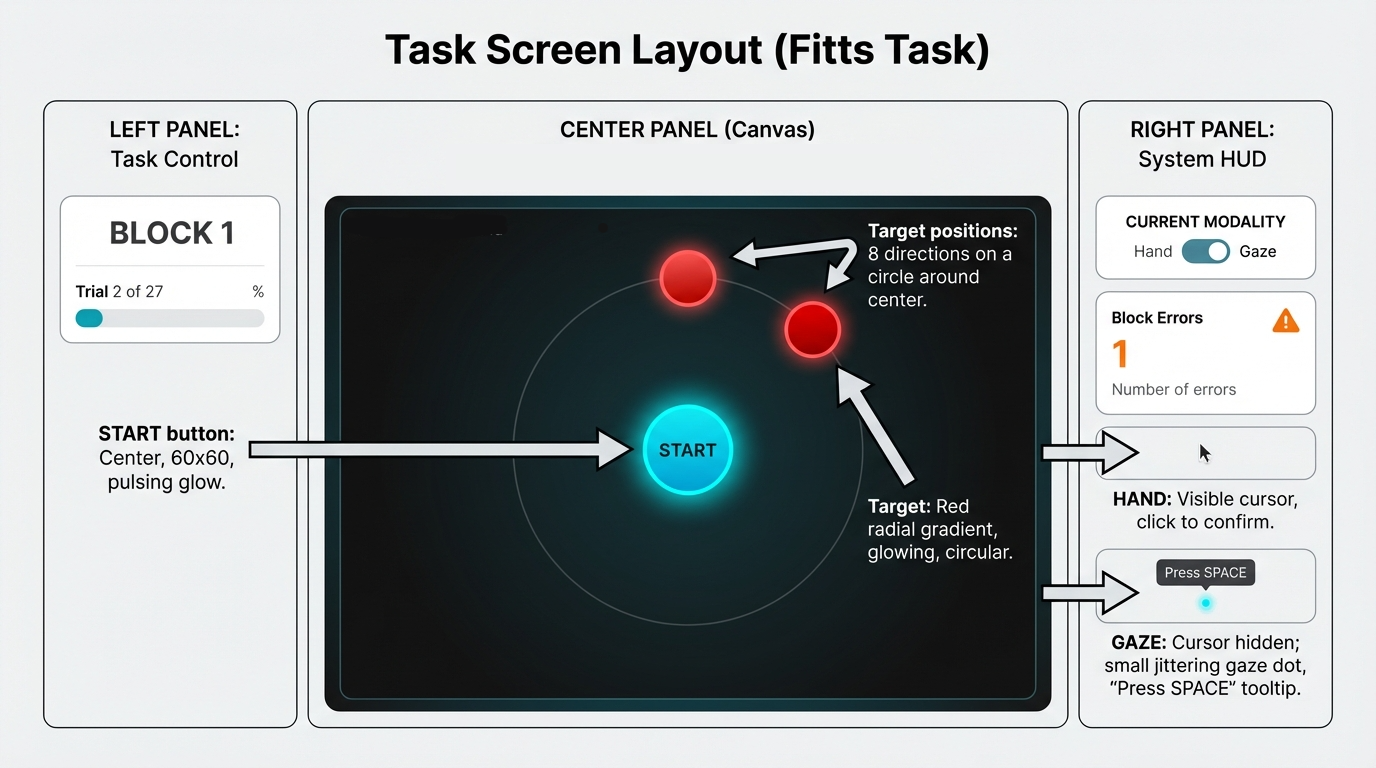
\includegraphics[width=0.85\linewidth,height=\textheight,keepaspectratio]{../assets/case_study/Task_layout.png}

}

\caption{\label{fig-task-layout}Task UI overview. ISO 9241-9
multi-directional tapping task: participants select highlighted targets
on a central canvas. A side HUD shows modality and block-level
feedback.}

\end{figure}%

\subsection{Experimental Design}\label{experimental-design}

We employed a repeated-measures factorial design: all participants
experienced every combination of the two input modalities (Gaze
vs.~Hand) × two UI conditions (Adaptive vs.~Non-adaptive) × two workload
levels (Pressure vs.~No Pressure). This creates a 2 × 2 × 2
within-subjects design.

\subsubsection{Counterbalancing: The Williams
Design}\label{counterbalancing-the-williams-design}

The order of modality blocks was counterbalanced using a Williams Latin
square arrangement to control for learning effects (Williams, 1949).
Static and adaptive conditions were run as \textbf{separate blocks};
each block corresponded to one Modality × UI Mode combination (e.g.,
Hand-Static, Gaze-Adaptive). Within each block, all trials shared the
same modality and UI mode. Participants were not explicitly told when
the system was adapting, aside from noticing the visual changes, to
reduce expectancy biases.

\subsection{Participants}\label{participants}

\subsubsection{Sample Size and
Recruitment}\label{sample-size-and-recruitment}

The planned confirmatory sample was N=48, corresponding to six complete
Williams counterbalancing blocks. At the time of this interim report,
the complete factorial dataset available for primary analysis included
N=23 participants. Seven earlier participants were excluded from the
primary 2 × 2 × 2 analysis because a pressure-logging bug misrecorded
block condition; their data were retained only for exploratory use.
Replacement recruitment is ongoing to restore the planned complete
sample of N=48. Participants were recruited from the university
community (target: balanced gender distribution, age range 18-35). All
had normal or corrected-to-normal vision and no known motor impairments.
The study was approved by the Institutional Review Board (IRB) and all
participants provided informed consent.

\subsection{Procedure}\label{procedure}

Each participant completed a short training session to get familiar with
gaze selection (including practice with the simulated gaze interface and
dwell clicking) and hand selection. During the experiment, they
performed 4 blocks of 40 trials each (160 trials total per participant).
Practice trials (10 per modality before the main blocks) were excluded
from analysis. Target positions cycled through 8 directions; Index of
Difficulty varied across three levels (\$\approx\$2--6 bits). Pressure
(time-limited vs.~self-paced) was varied within blocks.

After each block, participants filled out a NASA-TLX workload survey
(rating mental demand, physical demand, etc.) and took a short break to
mitigate fatigue. The entire session lasted about 1 hour per
participant.

\subsection{Measures and Analysis
Strategy}\label{measures-and-analysis-strategy}

The primary performance measures were Movement Time (MT) in milliseconds
(from trial start to successful selection) and Selection Accuracy (hit
vs.~miss rate, including specific error types). We classified errors
into three categories following Reason's (1990) taxonomy of human error:
\textbf{slips} (unintended activations---the cursor dwelled on a target
the user did not intend to select), \textbf{misses} (failures of spatial
targeting---the user attempted selection but did not acquire the target
within bounds), and \textbf{timeouts} (no response within the 6-second
trial window). From these, we computed Throughput (TP) in bits/second
for each condition by combining each trial's effective ID (\(ID_e\)) and
MT, following ISO 9241-9's recommended calculation using the effective
target width \(W_e\) (computed from the spread of hit points) to
incorporate accuracy into the difficulty measure.

Because this manuscript reports an interim dataset, the main text
emphasizes descriptive estimates and 95\% confidence intervals for the
currently available complete factorial sample. Confirmatory
mixed-effects models, preregistered contrasts, and
multiplicity-controlled follow-up tests will be reported after the
target sample of N=48 is reached. We adopted a \textbf{Hybrid Analysis}
framework to disentangle ``motor'' performance from ``decision''
caution: (1) \textbf{Macro-Performance (Fitts' Law)}---we modeled the
overall throughput (bits/s) and the regression slope (\(b\)) to quantify
the global cost of the gaze simulation lag, following standard ISO
9241-9 throughput calculations; (2) \textbf{Path Quality (Control
Theory)}---we logged velocity profiles and submovement counts for future
control-theory analysis; the present interim report focuses on
macro-performance and LBA; (3) \textbf{Decision Verification (LBA)}---we
used the Linear Ballistic Accumulator (LBA) model (Brown \& Heathcote,
2008) to analyze the verification phase (time from first target entry to
final selection). LBA is robust to low error rates and allows estimation
of non-decision time (NDT), drift rate, and decision threshold. We fit a
hierarchical Bayesian LBA model in PyMC with modality- and
UI-mode-varying NDT, ID-varying drift rate, and pressure-varying
threshold. For the verification-phase component, we used LBA rather than
DDM because the subset of trials used for that analysis did not provide
error patterns suitable for stable DDM estimation (Lerche et al., 2017).

\subsection{Deployment and Data Collection
Infrastructure}\label{deployment-and-data-collection-infrastructure}

The experimental platform was deployed as a web application (React 18,
TypeScript, Vite) hosted on Vercel
(https://xr-adaptive-modality-2025.vercel.app) to enable remote,
asynchronous data collection. Each participant received a unique URL
containing embedded participant ID and session number parameters (e.g.,
\texttt{?pid=P001\&session=1}). The application automatically detected
these parameters on load, initializing the session with the appropriate
identifier. Session state was managed client-side using browser
localStorage, enabling participants to pause and resume sessions while
maintaining progress tracking.

Data collection occurred entirely client-side to ensure participant
privacy. The application implemented a structured CSV logging system
that captured comprehensive trial-level data in real-time (77 columns
per trial), including participant metadata (ID, demographics, session
number), trial parameters (block, trial, modality, UI mode, pressure,
ID, A, W), performance metrics (RT, accuracy, error type, hover
duration, submovement count, verification time), adaptive system metrics
(width scaling, alignment gate metrics, adaptation triggers), system
metadata (browser type, DPR, display calibration, timestamp), and
workload measures (NASA-TLX subscales). At the completion of each
session, participants exported their data via browser-based CSV
download. Data export occurred entirely locally---no data was
transmitted to servers during the experimental session, ensuring
participant privacy. The application was built as a single-page
application (SPA) with client-side routing, with the gaze simulation
algorithm, adaptive policy engine, and data logging system all operating
in real-time within the browser. Event-driven architecture (via an
internal event bus) coordinated trial timing, data logging, and UI
updates, ensuring precise temporal alignment between user actions and
recorded data.

\textbf{Data Quality Assurance:} A comprehensive audit was conducted on
December 8, 2025, to verify data collection integrity. The audit
confirmed that modality and UI mode conditions were logged correctly (0
mismatches across all participants). However, a bug was identified in
the pressure condition logging that affected the first 7 participants
(see Participant Exclusions above). The bug was fixed immediately, and
all subsequent data collection used the corrected logging code. All code
is open-source and available for reproducibility.

\section{Results}\label{results}

We report interim results from the current dataset (N=23 participants
with complete factorial data). Full confirmatory analyses with
mixed-effects models will be reported upon completion of the target
sample (N=48).

\subsection{Primary Performance Outcomes
(RQ1)}\label{primary-performance-outcomes-rq1}

Throughput (TP), error rate, and movement time (MT) were computed
following ISO 9241-9. Table~\ref{tbl-performance} reports descriptive
statistics by modality, collapsed over UI mode and pressure.

\begin{longtable}[]{@{}lcc@{}}
\caption{Primary performance metrics by modality. Values are mean
{[}95\% CI{]}. Hand produced higher throughput and lower error rate than
gaze.}\label{tbl-performance}\tabularnewline
\toprule\noalign{}
Metric & Hand & Gaze \\
\midrule\noalign{}
\endfirsthead
\toprule\noalign{}
Metric & Hand & Gaze \\
\midrule\noalign{}
\endhead
\bottomrule\noalign{}
\endlastfoot
Throughput (bits/s) & 5.15 {[}5.06, 5.25{]} & 4.70 {[}4.56, 4.83{]} \\
Error Rate (\%) & 1.75 {[}1.23, 2.26{]} & 18.65 {[}17.26, 20.04{]} \\
Movement Time (s) & 1.09 {[}1.07, 1.11{]} & 1.19 {[}1.16, 1.23{]} \\
\end{longtable}

Hand input yielded higher throughput (5.15 vs.~4.70 bits/s) and
substantially lower error rate (1.75\% vs.~18.65\%) than gaze input.
Movement time was shorter for hand (1.09 s) than gaze (1.19 s).
Descriptively, hand outperformed gaze on throughput and error rate in
the current complete-case dataset. Figure~\ref{fig-performance}
illustrates these differences.

\begin{figure}[H]

\centering{

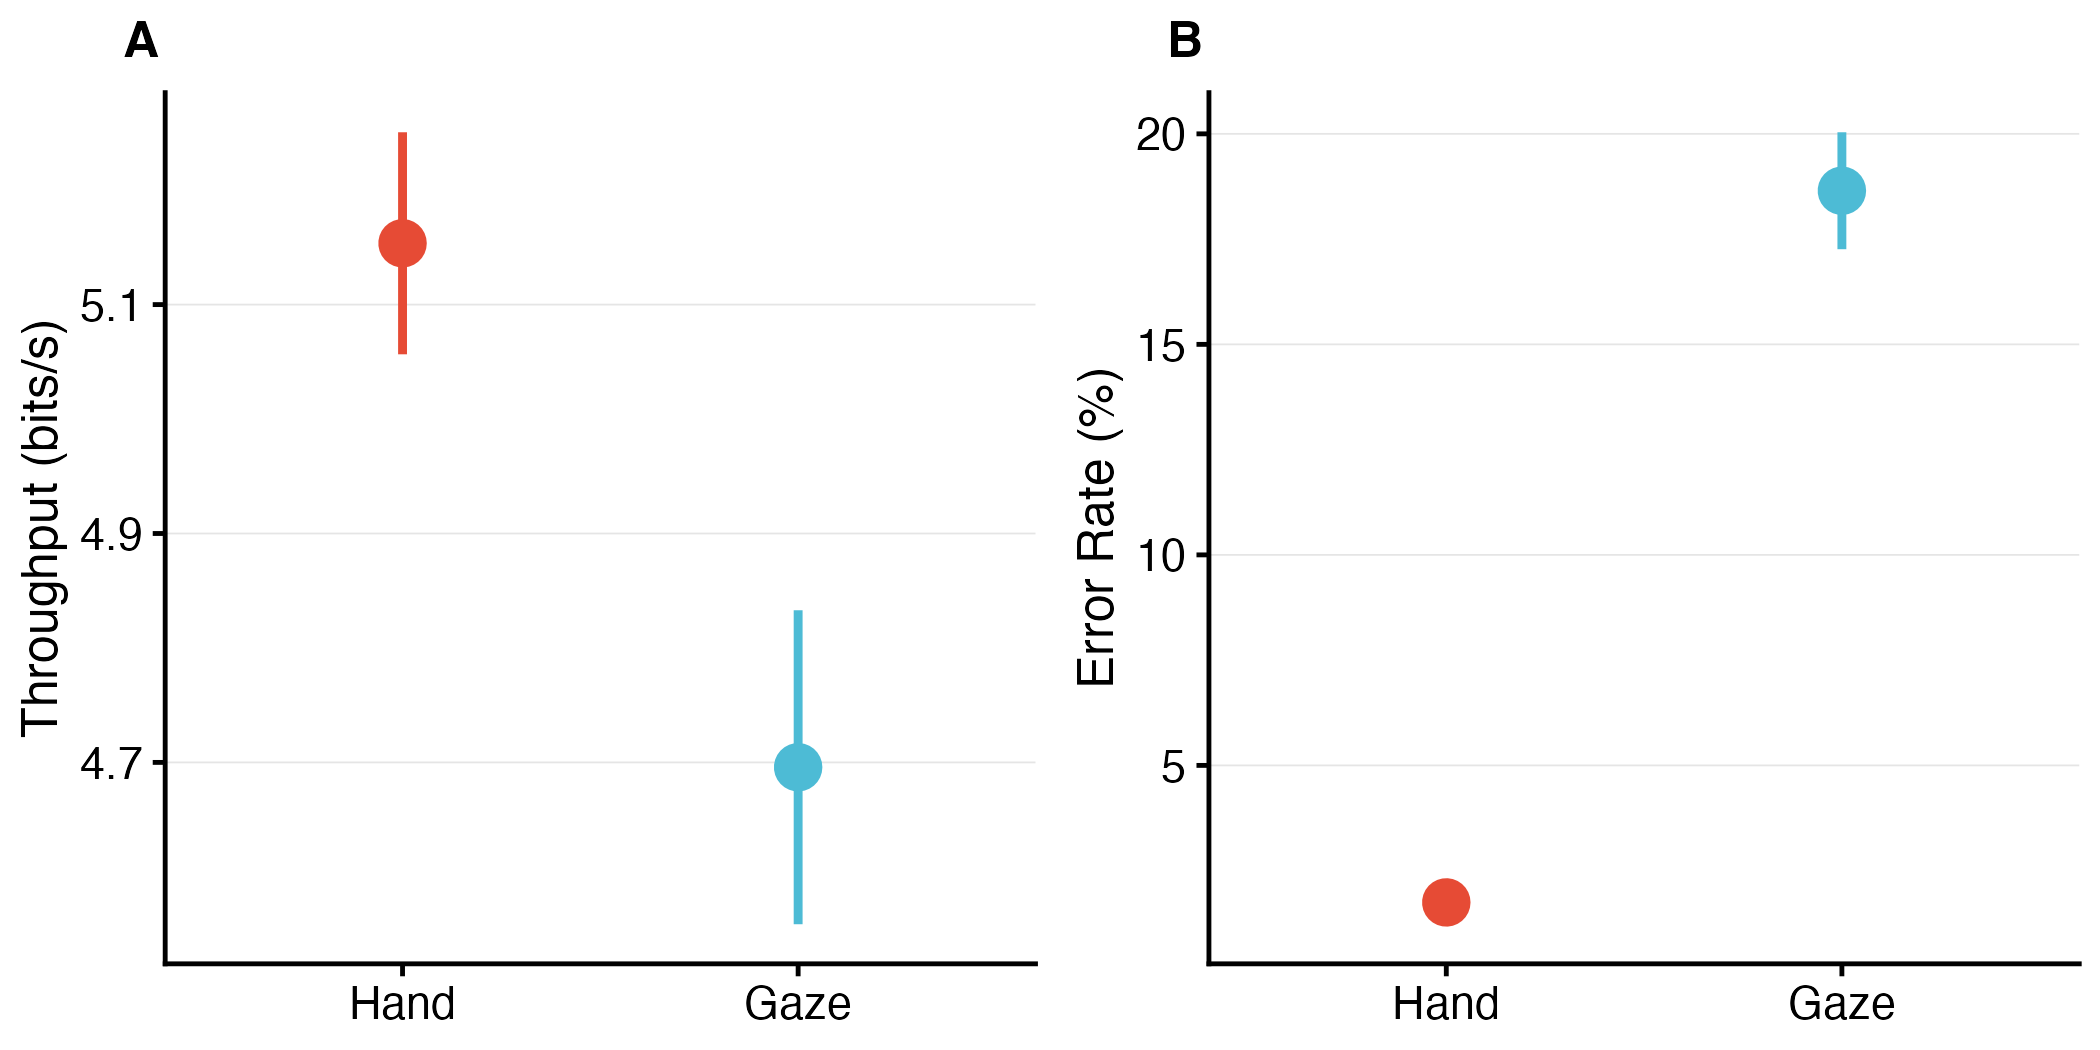
\includegraphics[width=0.85\linewidth,height=\textheight,keepaspectratio]{../assets/case_study/performance_combined.png}

}

\caption{\label{fig-performance}Primary performance by modality. (A)
Throughput (bits/s): hand produced higher throughput than gaze. (B)
Error rate (\%): gaze showed substantially higher error rate than hand.
Error bars show 95\% CI.}

\end{figure}%

\subsection{Error Profile: Midas Touch
Signature}\label{error-profile-midas-touch-signature}

Error types differed sharply between modalities
(Table~\ref{tbl-error-types}). For \textbf{gaze}, 99.2\% of errors were
\textbf{slips} (accidental activations) and 0.8\% were timeouts. For
\textbf{hand}, 95.7\% were \textbf{misses} (target not acquired) and
4.3\% were timeouts. This asymmetry strongly supports the Midas Touch
account (Jacob, 1990): gaze interaction failed primarily due to intent
ambiguity (looking to see vs.~looking to select), whereas hand
interaction failed due to spatial targeting errors.

\begin{longtable}[]{@{}lcc@{}}
\caption{Distribution of error types by modality. Gaze errors are
predominantly slips; hand errors are predominantly
misses.}\label{tbl-error-types}\tabularnewline
\toprule\noalign{}
Error Type & Hand & Gaze \\
\midrule\noalign{}
\endfirsthead
\toprule\noalign{}
Error Type & Hand & Gaze \\
\midrule\noalign{}
\endhead
\bottomrule\noalign{}
\endlastfoot
Slip (accidental activation) & 0\% & 99.2\% \\
Miss (target not acquired) & 95.7\% & 0\% \\
Timeout & 4.3\% & 0.8\% \\
\end{longtable}

Figure~\ref{fig-error-types} shows the composition of errors by
modality, illustrating the stark contrast between gaze (slips) and hand
(misses).

\begin{figure}[H]

\centering{


\includegraphics[width=0.75\linewidth,height=\textheight,keepaspectratio]{../assets/case_study/error_type_composition.png}

}

\caption{\label{fig-error-types}Error type composition by modality. Gaze
errors are predominantly slips (accidental activations); hand errors are
predominantly misses.}

\end{figure}%

\subsection{Gaze Declutter Effectiveness
(RQ3)}\label{gaze-declutter-effectiveness-rq3}

The gaze adaptive manipulation (declutter) was the only adaptation that
executed in this dataset. Gaze error rate was modestly lower in adaptive
(18.2\%) than static (19.1\%) mode. The declutter mechanism reduced
timeouts (1.18\% → 0.42\%) but did not materially reduce slips (98.8\% →
99.6\%). Hand width inflation was not evaluable in the present dataset
(width scaling remained at 1.0; see Appendix). At N=23, the declutter
effect is directional; confirmatory tests will be reported at N=48.

\subsection{Subjective Workload (RQ2)}\label{subjective-workload-rq2}

NASA-TLX scores (0--100) were higher for gaze than hand across all
subscales (Table~\ref{tbl-tlx}). Overall workload (unweighted mean of
six subscales) was 40.4 {[}37.0, 43.8{]} for hand and 47.0 {[}43.9,
50.2{]} for gaze. For the RQ2-specified subscales, \textbf{Physical
Demand} was 34.3 {[}30.8, 37.8{]} (hand) vs.~41.9 {[}38.4, 45.4{]}
(gaze), and \textbf{Frustration} was 32.2 {[}28.5, 35.9{]} (hand)
vs.~43.2 {[}39.5, 46.9{]} (gaze).

\begin{longtable}[]{@{}lcc@{}}
\caption{NASA-TLX subscale means {[}95\% CI{]} by modality. Higher =
more workload.}\label{tbl-tlx}\tabularnewline
\toprule\noalign{}
NASA-TLX Subscale & Hand & Gaze \\
\midrule\noalign{}
\endfirsthead
\toprule\noalign{}
NASA-TLX Subscale & Hand & Gaze \\
\midrule\noalign{}
\endhead
\bottomrule\noalign{}
\endlastfoot
Mental Demand & 34.9 {[}31.5, 38.4{]} & 45.7 {[}42.4, 49.1{]} \\
Physical Demand & 34.3 {[}30.8, 37.8{]} & 41.9 {[}38.4, 45.4{]} \\
Temporal Demand & 40.3 {[}36.9, 43.6{]} & 47.1 {[}44.0, 50.1{]} \\
Performance & 55.6 {[}50.4, 60.9{]} & 53.3 {[}49.3, 57.3{]} \\
Effort & 39.8 {[}36.1, 43.5{]} & 48.6 {[}45.2, 51.9{]} \\
Frustration & 32.2 {[}28.5, 35.9{]} & 43.2 {[}39.5, 46.9{]} \\
\textbf{Overall} & \textbf{40.4 {[}37.0, 43.8{]}} & \textbf{47.0
{[}43.9, 50.2{]}} \\
\end{longtable}

Figure~\ref{fig-tlx} shows overall workload by modality.
Figure~\ref{fig-tlx-subscales} compares workload across the six NASA-TLX
subscales, making it clear which dimensions (e.g., Physical Demand,
Frustration) differ most between hand and gaze.

\begin{figure}[H]

\centering{

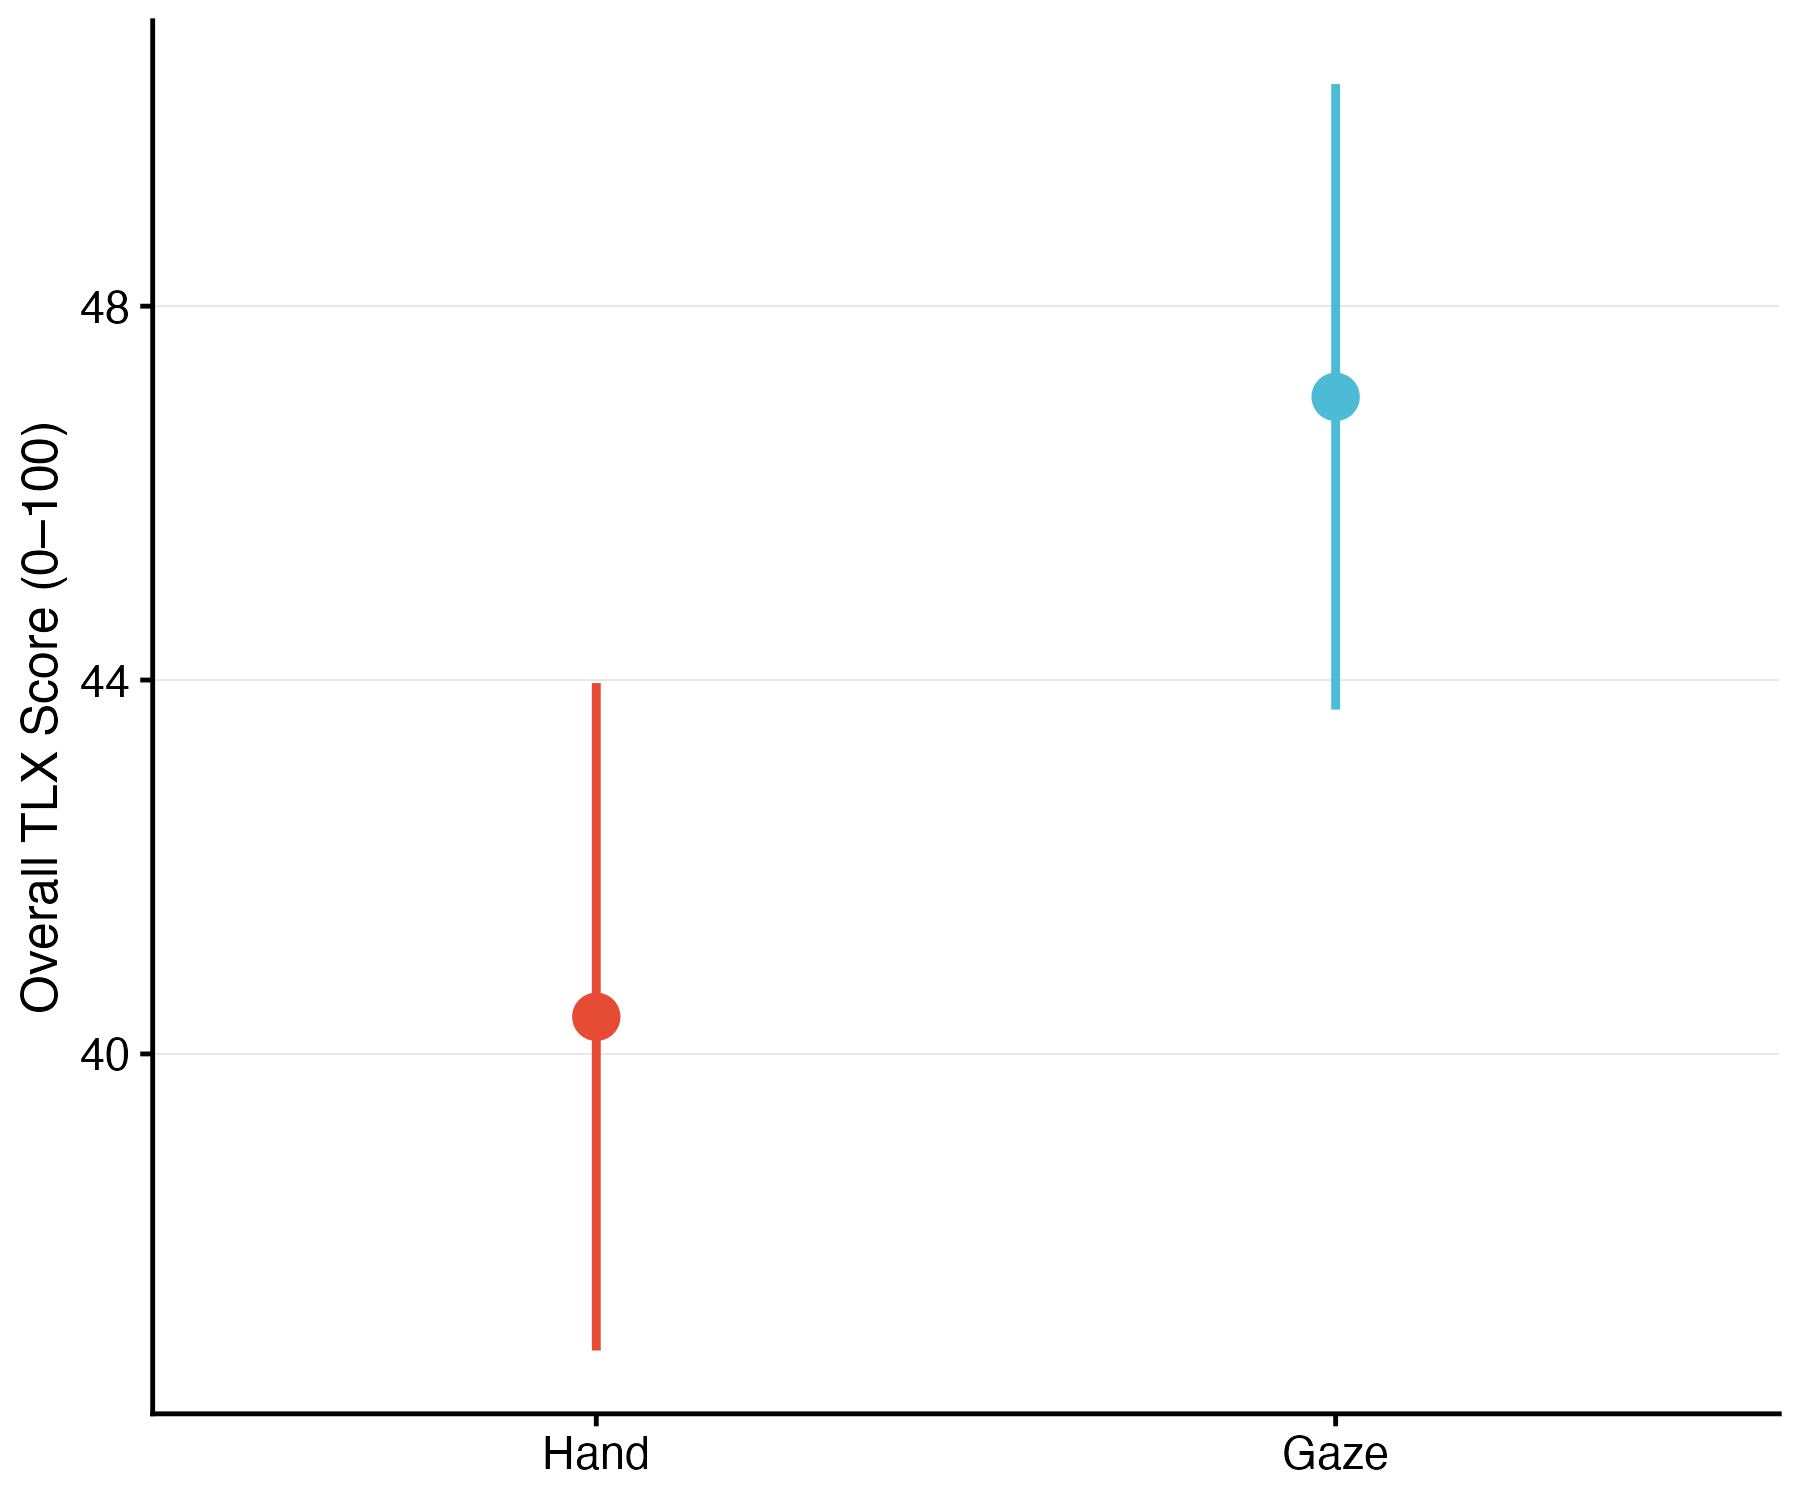
\includegraphics[width=0.7\linewidth,height=\textheight,keepaspectratio]{../assets/case_study/tlx_overall.png}

}

\caption{\label{fig-tlx}NASA-TLX overall workload (0--100) by modality.
Gaze imposed higher subjective workload than hand. Error bars show 95\%
CI.}

\end{figure}%

\begin{figure}[H]

\centering{

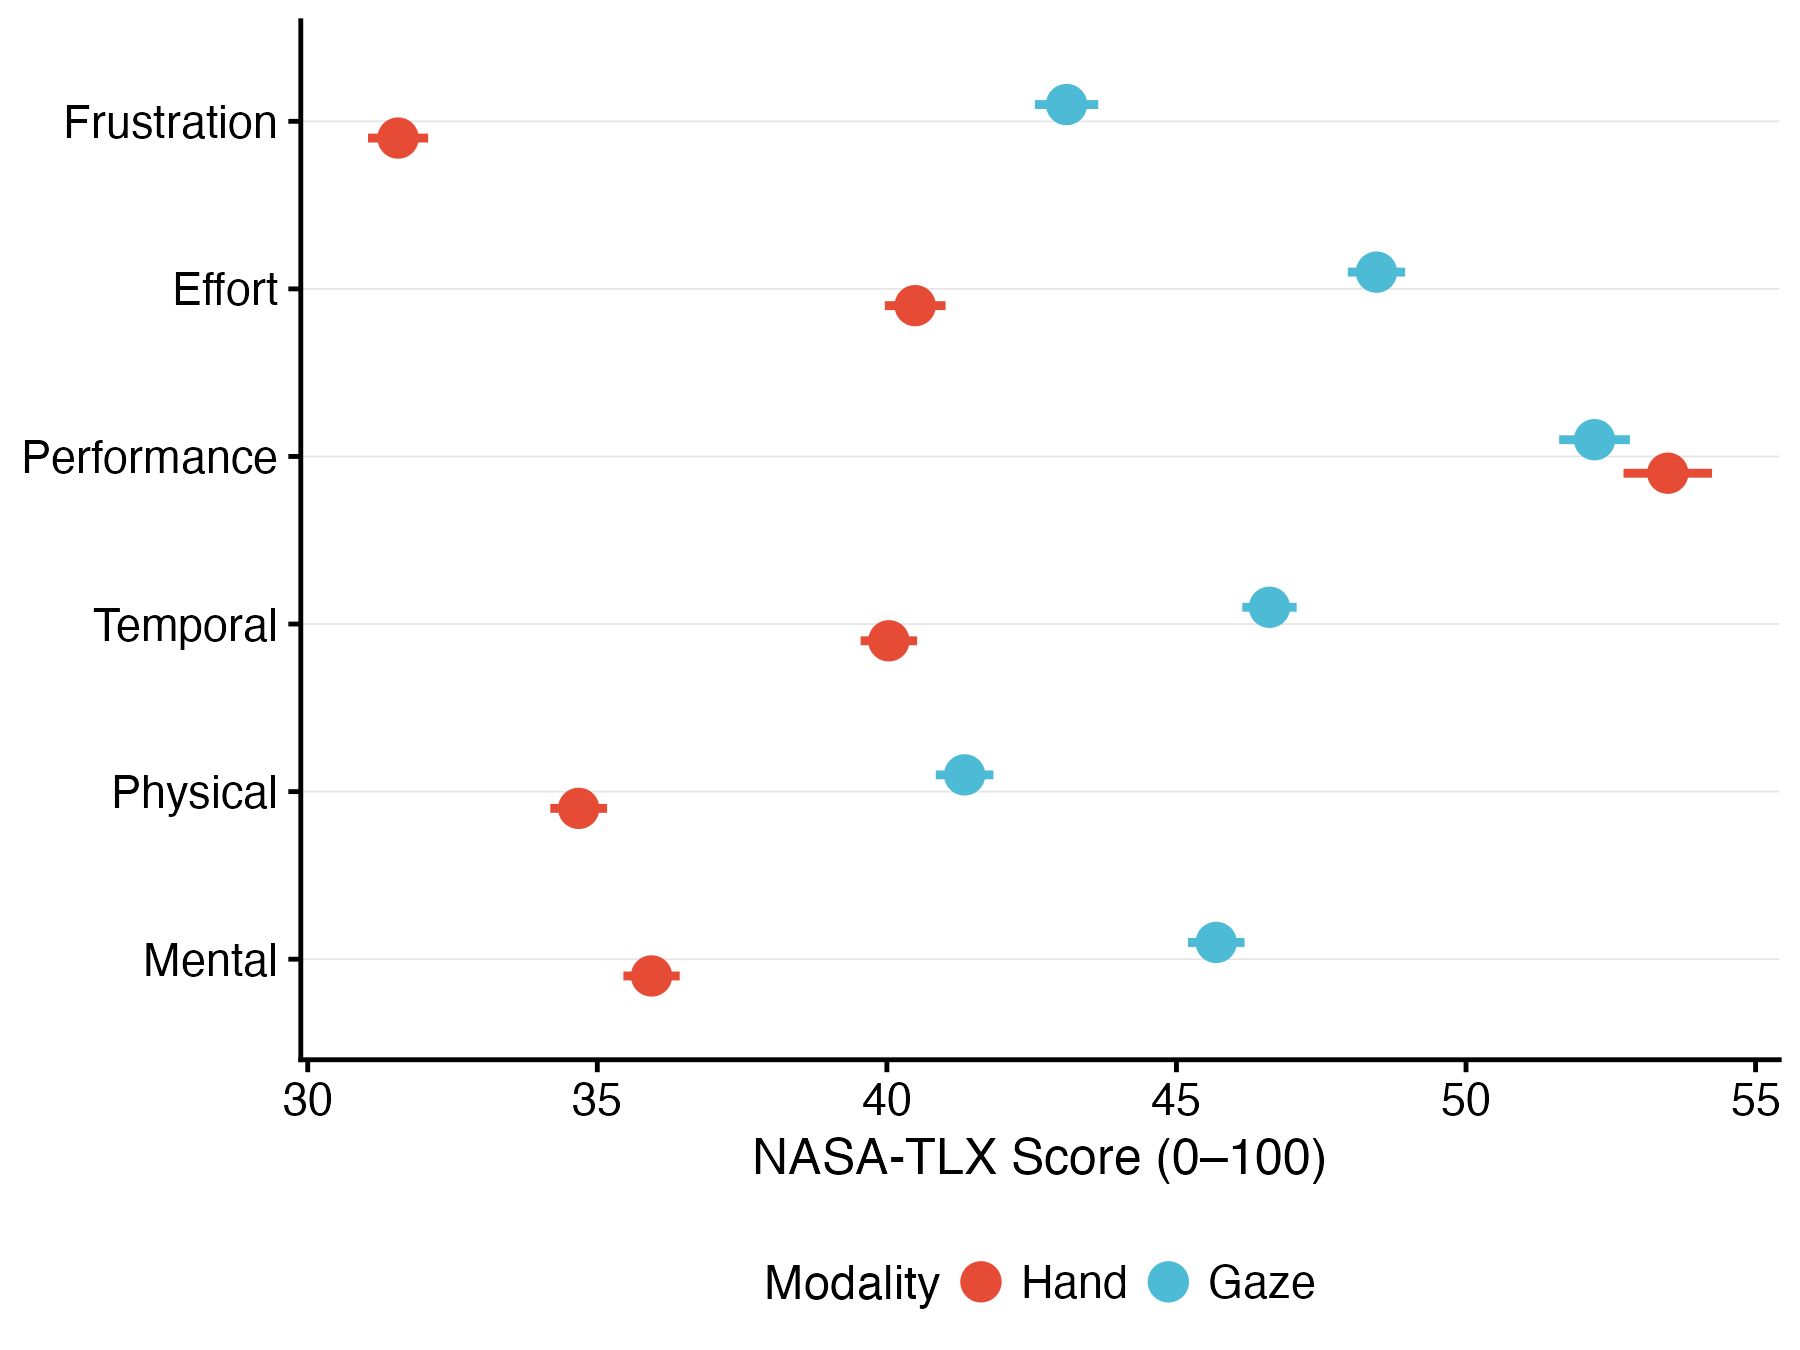
\includegraphics[width=0.75\linewidth,height=\textheight,keepaspectratio]{../assets/case_study/tlx_subscales.png}

}

\caption{\label{fig-tlx-subscales}NASA-TLX subscales by modality.
Point-range plot comparing Hand and Gaze on each subscale (Mental,
Physical, Temporal, Performance, Effort, Frustration). Gaze shows higher
scores on most dimensions; Physical Demand and Frustration show the
largest modality differences. Error bars show 95\% CI.}

\end{figure}%

\subsection{LBA Cognitive Modeling}\label{lba-cognitive-modeling}

The LBA model decomposes verification-phase reaction time into latent
cognitive components: \textbf{non-decision time} (NDT, encoding + motor
execution), \textbf{drift rate} (information accumulation speed), and
\textbf{decision threshold} (caution). We fit a hierarchical Bayesian
LBA model in PyMC, with NDT varying by modality and UI mode, drift rate
varying by Index of Difficulty (ID), and threshold varying by pressure
condition. The model used verification-phase RTs (200--5000 ms) from
valid trials. MCMC sampling used multiple chains with R-hat \textless{}
1.01 and ESS \textgreater{} 2,000 for all parameters, indicating
convergence.

\subsubsection{Parameter Estimates}\label{parameter-estimates}

Table~\ref{tbl-lba-params} reports group-level LBA parameter estimates
by modality and UI mode. Non-decision time (t0) is the primary parameter
that varies across conditions; drift and threshold parameters are shared
across conditions with modality- and pressure-specific effects captured
in the hierarchical structure. Figure~\ref{fig-lba-t0} visualizes the t0
posterior estimates and 95\% HDIs by condition, making the modality and
UI-mode differences immediately apparent: gaze conditions show higher
(less negative) t0 values than hand conditions, indicating longer
verification-phase duration. Figure~\ref{fig-verification-rt} shows the
empirical verification-phase RT by condition, bridging the raw observed
behavior to the modeled latent parameters.

\begin{longtable}[]{@{}
  >{\raggedright\arraybackslash}p{(\linewidth - 8\tabcolsep) * \real{0.1111}}
  >{\centering\arraybackslash}p{(\linewidth - 8\tabcolsep) * \real{0.2333}}
  >{\centering\arraybackslash}p{(\linewidth - 8\tabcolsep) * \real{0.1333}}
  >{\centering\arraybackslash}p{(\linewidth - 8\tabcolsep) * \real{0.2333}}
  >{\centering\arraybackslash}p{(\linewidth - 8\tabcolsep) * \real{0.2889}}@{}}
\caption{LBA parameter estimates by modality and UI mode. Point
estimates with 95\% highest-density intervals. t0 (latent): non-decision
time; higher values indicate longer verification-phase duration. ID
slope: effect of difficulty on drift (negative = harder trials reduce
drift). Pressure slope: effect of time pressure on threshold. Drift base
and threshold intercept shared across
conditions.}\label{tbl-lba-params}\tabularnewline
\toprule\noalign{}
\begin{minipage}[b]{\linewidth}\raggedright
Condition
\end{minipage} & \begin{minipage}[b]{\linewidth}\centering
t0 (NDT) {[}95\% HDI{]}
\end{minipage} & \begin{minipage}[b]{\linewidth}\centering
Drift Base
\end{minipage} & \begin{minipage}[b]{\linewidth}\centering
ID Slope {[}95\% HDI{]}
\end{minipage} & \begin{minipage}[b]{\linewidth}\centering
Pressure Slope {[}95\% HDI{]}
\end{minipage} \\
\midrule\noalign{}
\endfirsthead
\toprule\noalign{}
\begin{minipage}[b]{\linewidth}\raggedright
Condition
\end{minipage} & \begin{minipage}[b]{\linewidth}\centering
t0 (NDT) {[}95\% HDI{]}
\end{minipage} & \begin{minipage}[b]{\linewidth}\centering
Drift Base
\end{minipage} & \begin{minipage}[b]{\linewidth}\centering
ID Slope {[}95\% HDI{]}
\end{minipage} & \begin{minipage}[b]{\linewidth}\centering
Pressure Slope {[}95\% HDI{]}
\end{minipage} \\
\midrule\noalign{}
\endhead
\bottomrule\noalign{}
\endlastfoot
Hand -- Static & −2.85 {[}−3.46, −2.24{]} & 5.03 & −0.93 {[}−0.95,
−0.92{]} & 0.06 {[}0.03, 0.09{]} \\
Hand -- Adaptive & −3.01 {[}−3.64, −2.42{]} & 5.03 & −0.93 {[}−0.95,
−0.92{]} & 0.06 {[}0.03, 0.09{]} \\
Gaze -- Static & −1.41 {[}−1.87, −1.00{]} & 5.03 & −0.93 {[}−0.95,
−0.92{]} & 0.06 {[}0.03, 0.09{]} \\
Gaze -- Adaptive & −0.97 {[}−1.39, −0.57{]} & 5.03 & −0.93 {[}−0.95,
−0.92{]} & 0.06 {[}0.03, 0.09{]} \\
\end{longtable}

\begin{figure}[H]

\centering{

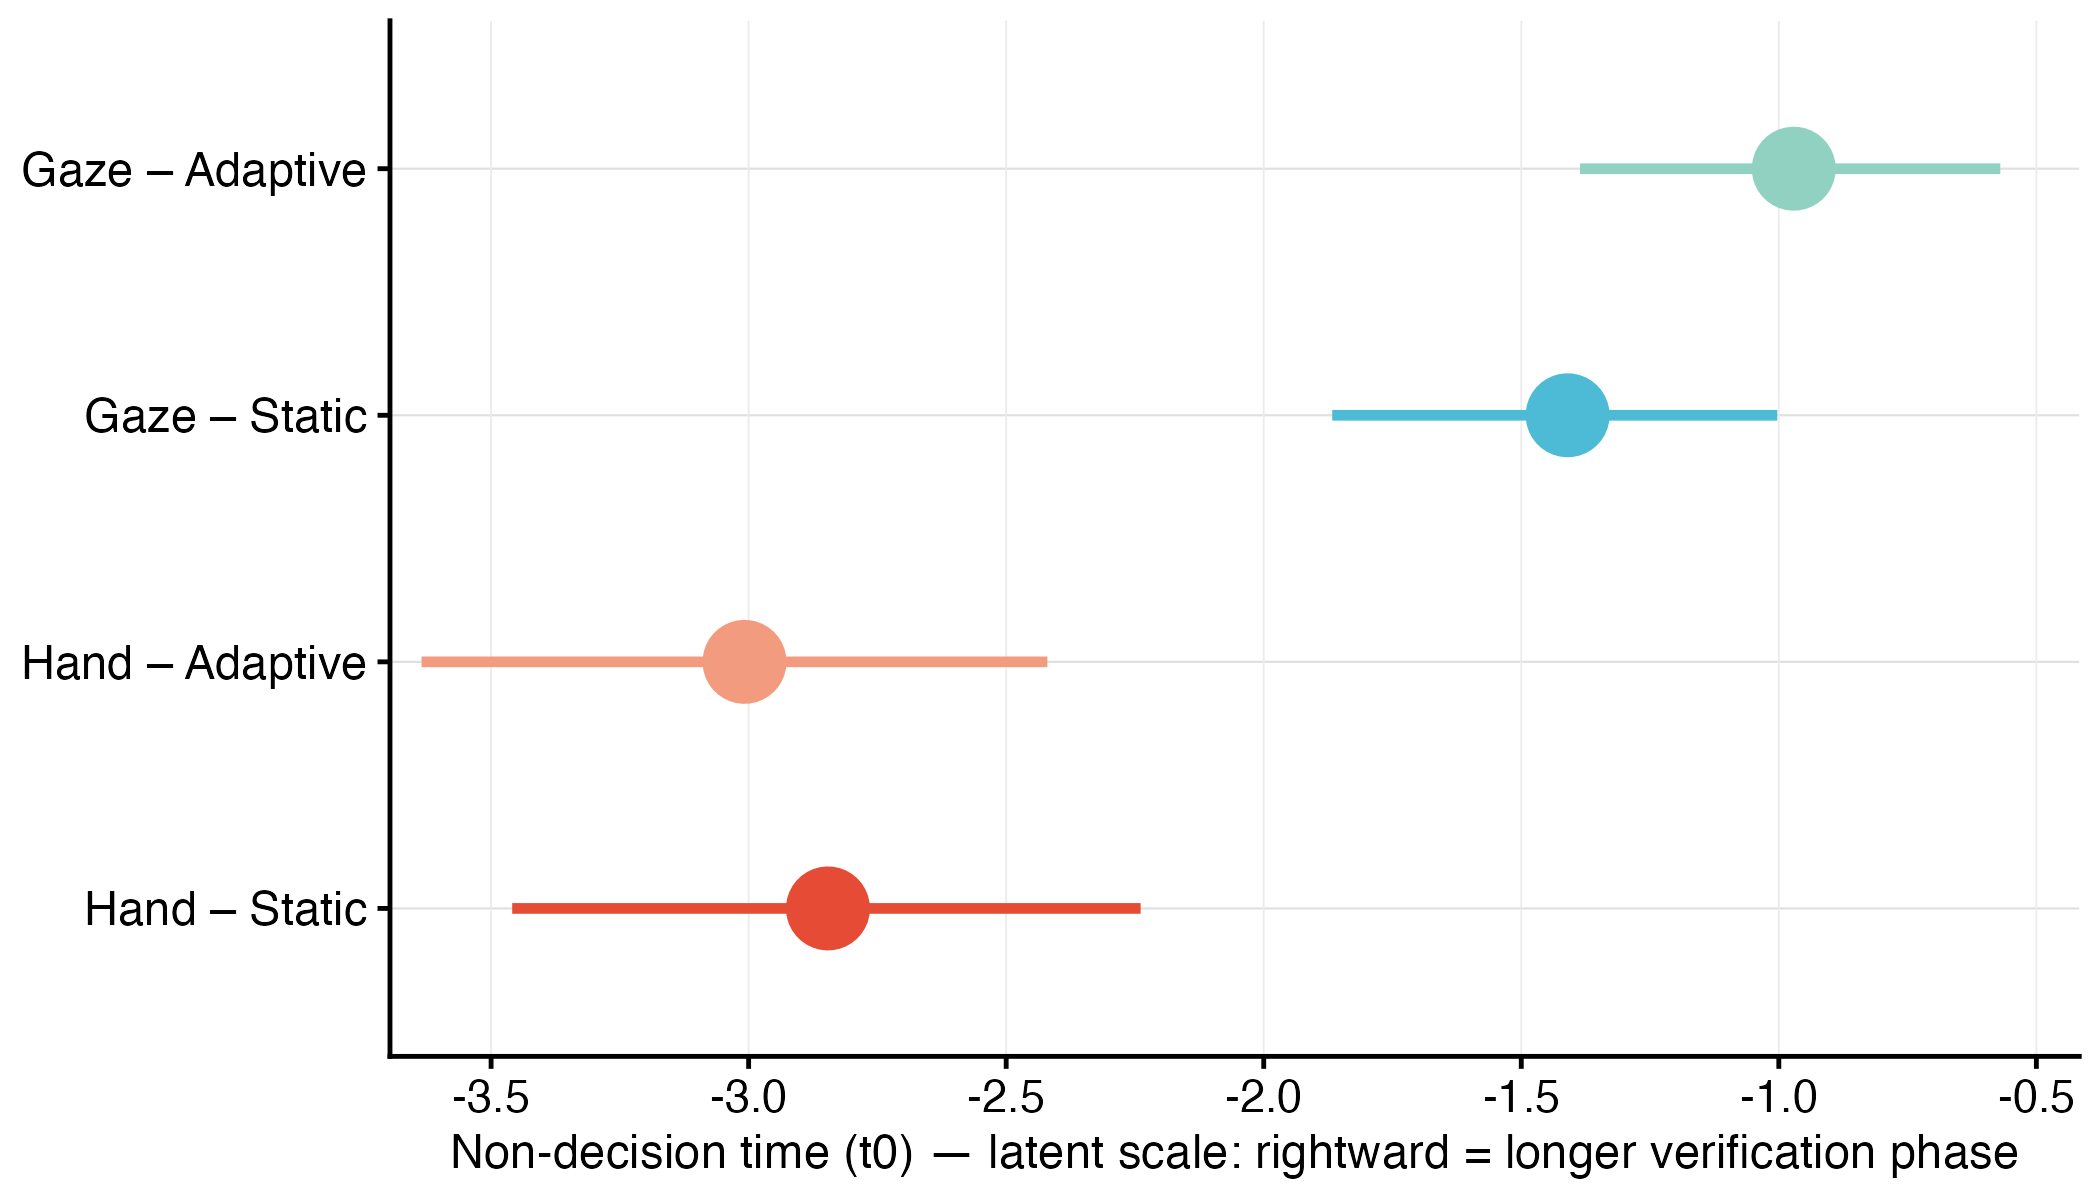
\includegraphics[width=0.9\linewidth,height=\textheight,keepaspectratio]{../assets/case_study/lba_t0_forest.png}

}

\caption{\label{fig-lba-t0}Non-decision time (t0) by condition. Each row
shows one condition; the point is the posterior mean and the horizontal
line is the 95\% highest-density interval. t0 is the time spent on
encoding and motor execution before the decision process---the
verification phase. Values are on a latent scale (negative); rightward
means longer verification phase. Gaze conditions (top two rows) show
longer t0 than hand conditions (bottom two rows), meaning gaze required
more time before users committed to selection---consistent with the
Midas Touch problem.}

\end{figure}%

\begin{figure}[H]

\centering{

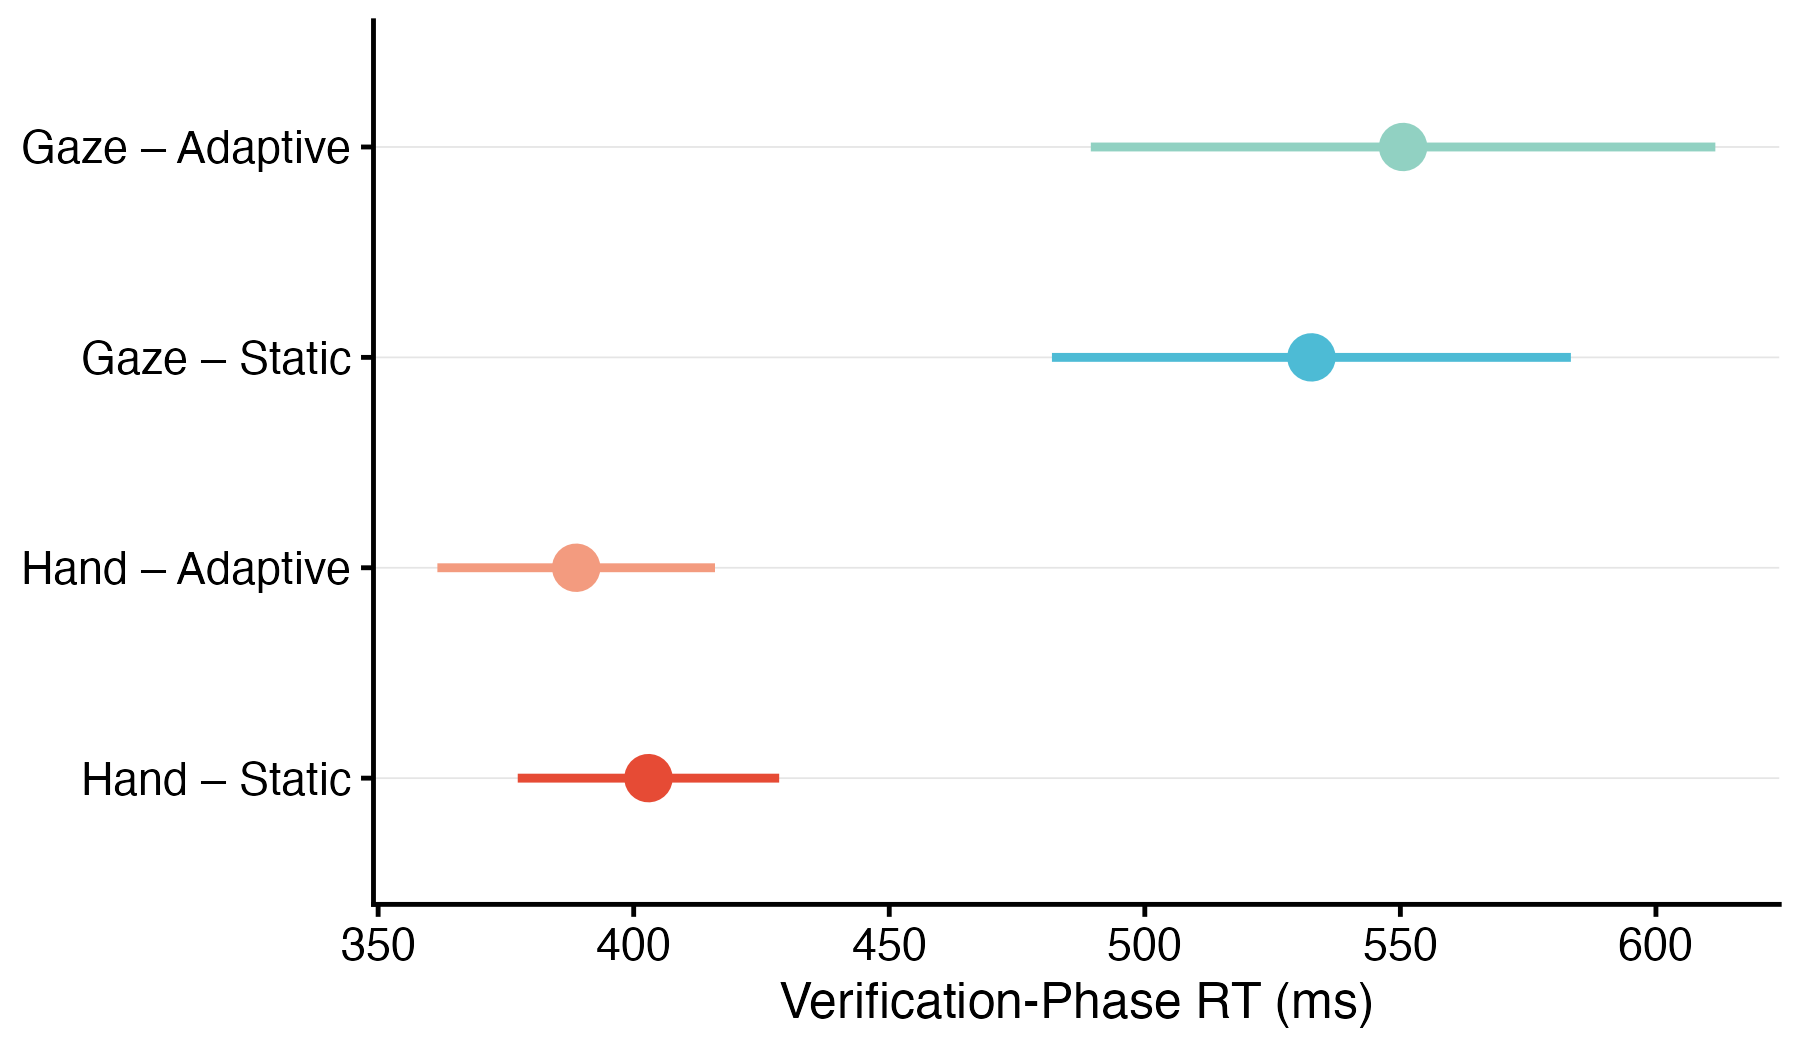
\includegraphics[width=0.85\linewidth,height=\textheight,keepaspectratio]{../assets/case_study/verification_rt_empirical.png}

}

\caption{\label{fig-verification-rt}Empirical verification-phase RT by
condition. Mean verification time (ms) from first target entry to
selection, with 95\% CI. Bridges the raw observed behavior to the
LBA-modeled latent parameters.}

\end{figure}%

\subsubsection{Interpretation}\label{interpretation}

\textbf{Modality effect on NDT:} Gaze conditions show higher t0 values
(less negative: −1.41 to −0.97) than hand conditions (−3.01 to −2.85),
consistent with a longer verification-phase duration for gaze
interaction. The pattern is compatible with the Midas Touch account:
gaze may require additional time for intent disambiguation before
selection.

\textbf{UI mode effect:} Adaptive UI shows different t0 patterns,
particularly for gaze (static: −1.41, adaptive: −0.97). The higher t0 in
gaze-adaptive may reflect altered verification timing under declutter,
though the direction warrants further investigation with the full
sample.

\textbf{Difficulty and pressure:} The negative ID slope (−0.93) is
consistent with harder trials reducing drift rate (Fitts's Law). The
positive pressure slope (0.06) suggests a speed--accuracy tradeoff:
higher time pressure increases the decision threshold.

\subsubsection{Convergence Diagnostics}\label{convergence-diagnostics}

MCMC convergence was satisfactory: R-hat remained at 1.0 for all
parameters, and ESS exceeded 2,000. The drift-rate slope (ID) and
threshold slope (pressure) exhibited unimodal posteriors and well-mixed
chains. Non-decision time showed multiple modes across the four
condition cells, reflecting the hierarchical structure. Trace plots are
provided in the Appendix (Figure~\ref{fig-lba-trace}).

\section{Discussion}\label{discussion}

The interim results suggest a clear modality asymmetry in XR pointing
performance. Across the primary performance measures, hand input
outperformed gaze input: hand produced higher throughput (5.15 vs.~4.70
bits/s), lower error (1.75\% vs.~18.65\%), and shorter movement time
(1.09 vs.~1.19 s). The workload pattern paralleled these performance
differences. NASA-TLX scores were higher for gaze than hand overall
(47.0 vs.~40.4), with especially notable differences in Physical Demand
(41.9 vs.~34.3) and Frustration (43.2 vs.~32.2). Taken together, these
interim findings address RQ1 and RQ2 in a consistent direction: under
the present task and simulation conditions, gaze interaction was not
merely less accurate than hand input, but also experienced as more
effortful.

The most informative result is not only that gaze performed worse, but
how it failed. Gaze errors were overwhelmingly slips (99.2\%), whereas
hand errors were overwhelmingly misses (95.7\%). This asymmetry is
important because it distinguishes two different failure regimes. Hand
failures reflected spatial targeting difficulty: users attempted the
correct action but failed to acquire the target. Gaze failures instead
reflected intent ambiguity: the system registered activation when users
were looking, but not necessarily intending to select. This pattern is
directly consistent with the Midas Touch account proposed by Jacob
(1990). In that sense, the present dataset contributes more than another
hand-versus-gaze comparison. It shows that the principal liability of
gaze in this XR task was not generic imprecision alone, but the coupling
of visual attention and command execution.

These findings also fit the information-theoretic interpretation of
pointing performance formalized by Fitts's Law (Soukoreff \& MacKenzie,
2004). Throughput reflects the effective rate at which a user can
resolve spatial uncertainty, expressed in bits per second. On that
metric, hand preserved a higher information-processing rate than gaze in
the current task. The appendix-level Fitts validation supports this
interpretation: hand showed stronger fits and more stable scaling with
index of difficulty, whereas gaze exhibited weaker fits and lower
explained variance. Although both modalities were affected by task
difficulty, the flatter and noisier gaze fits suggest that its
performance was shaped by more than ballistic movement alone. In other
words, increasing difficulty did not simply elongate transport time; it
also appears to have amplified downstream verification demands.

The cognitive modeling results sharpen that interpretation. In the LBA
analysis, gaze showed higher non-decision time than hand, indicating a
longer pre- or post-decisional component surrounding overt selection
(Brown \& Heathcote, 2008). In the present task, the most plausible
interpretation is that gaze required a longer verification phase before
commitment. That is exactly where a Midas Touch problem should appear:
not necessarily in the initial orientation toward a target, but in the
added delay needed to decide whether fixation is sufficiently stable,
intentional, and safe to confirm. The negative ID slope for drift rate
(−0.93) is also consistent with a Fitts-like account in which harder
trials reduce the rate of evidence accumulation. The positive pressure
slope (0.06) further suggests that time pressure altered the caution
policy rather than simply speeding responses, which is consistent with a
speed--accuracy tradeoff account. Taken together, the LBA results
indicate that gaze interaction imposed a verification burden beyond raw
target acquisition.

This pattern can also be understood through the lens of cognitive load.
In principle, gaze offers a low-effort means of orienting to targets,
while hand input incurs greater bodily effort, especially in spatial
interfaces often associated with ``Gorilla Arm'' fatigue. Yet the
present workload results suggest that, in this task, gaze introduced
greater extraneous load than hand. That load likely came from the need
to monitor cursor stability, manage dwell or confirmation timing, and
suppress unintended selections. Hand input, by contrast, appears to have
shifted the burden toward controlled spatial targeting, but in a way
that remained more manageable under the current task constraints. In
that sense, the gaze--hand tradeoff is not well captured by a simple
speed-versus-fatigue dichotomy. Rather, gaze may reduce some motor
demands while increasing decisional and attentional overhead; hand may
require more overt motor control while preserving clearer action
intention and lower ambiguity. The workload findings are consistent with
that framing, particularly the elevated Frustration scores under gaze.

RQ3 received only partial support in this interim dataset. The only
adaptive mechanism that actually executed was gaze declutter, and its
benefit was modest. Gaze error declined directionally from 19.1\% in the
static condition to 18.2\% in the adaptive condition. More specifically,
declutter reduced timeouts from 1.18\% to 0.42\%, but did not reduce
slips; slips remained dominant and even slightly increased
proportionally (98.8\% to 99.6\%). This pattern suggests that declutter
may have helped with distraction-driven hesitation or delayed
commitment, but it did not address the core failure mode of gaze
interaction, namely intent disambiguation. That distinction matters: if
the main problem is that users accidentally activate while looking,
reducing peripheral clutter may improve attentional focus without
solving the actual selection ambiguity. By contrast, the hand
width-inflation mechanism was not evaluable in the present dataset
(width scaling remained at 1.0; the policy engine emitted actions in
some sessions but the UI did not apply them to rendered targets). Any
interpretation of RQ3 must therefore remain provisional until the full
confirmatory sample is collected and both adaptation pathways are
observed in operation.

The present findings are broadly aligned with prior work showing both
the promise and fragility of gaze-based interaction in multimodal
systems. Prior gaze+hand paradigms have often treated gaze as an
efficient means of target acquisition and the hand as a confirmation or
refinement channel, thereby exploiting the complementary strengths of
the two modalities (Pfeuffer et al., 2017). That general logic is
compatible with the current results: gaze appears efficient for
orienting attention, but unreliable as a sole selection mechanism when
intent must be inferred from fixation. Likewise, the width-inflation
mechanism draws conceptually on expanding-target and Bubble Cursor work,
which has repeatedly shown that increasing effective target size can
improve pointing performance under uncertainty (Grossman \&
Balakrishnan, 2005; McGuffin \& Balakrishnan, 2005). A key contribution
of the present platform is the integration of physiologically
constrained gaze simulation, an ISO 9241-9 task structure, and
policy-driven adaptive modality logic within one reproducible framework.
That combination makes it possible to study modality-specific failure
modes under controlled conditions rather than treating gaze and hand as
interchangeable input channels.

The design implications are practical. For XR designers, the current
interim evidence suggests that hand input remains the more reliable
option for precise selection tasks in which slips are costly. Gaze may
still be valuable for rapid orienting, scanning, or coarse target
acquisition, but only when paired with a mechanism that resolves intent
ambiguity. Declutter may help when performance degradation is driven by
visual competition or hesitation, but it is unlikely to solve Midas
Touch on its own. More generally, adaptive systems in XR should not be
judged only by whether adaptation occurred, but by whether the
adaptation targets the dominant failure mode of the modality.
Table~\ref{tbl-design-implications} summarizes these modality-specific
guidelines.

\begin{longtable}[]{@{}
  >{\raggedright\arraybackslash}p{(\linewidth - 4\tabcolsep) * \real{0.1724}}
  >{\raggedright\arraybackslash}p{(\linewidth - 4\tabcolsep) * \real{0.3966}}
  >{\raggedright\arraybackslash}p{(\linewidth - 4\tabcolsep) * \real{0.4310}}@{}}
\caption{Design implications: modality-specific failure modes and
recommended adaptive
interventions.}\label{tbl-design-implications}\tabularnewline
\toprule\noalign{}
\begin{minipage}[b]{\linewidth}\raggedright
Modality
\end{minipage} & \begin{minipage}[b]{\linewidth}\raggedright
Dominant Failure Mode
\end{minipage} & \begin{minipage}[b]{\linewidth}\raggedright
Recommended Adaptation
\end{minipage} \\
\midrule\noalign{}
\endfirsthead
\toprule\noalign{}
\begin{minipage}[b]{\linewidth}\raggedright
Modality
\end{minipage} & \begin{minipage}[b]{\linewidth}\raggedright
Dominant Failure Mode
\end{minipage} & \begin{minipage}[b]{\linewidth}\raggedright
Recommended Adaptation
\end{minipage} \\
\midrule\noalign{}
\endhead
\bottomrule\noalign{}
\endlastfoot
Gaze & Slips (unintended activation) & Declutter for distraction-driven
hesitation; intent disambiguation (dwell, confirmation) for core Midas
Touch \\
Hand & Misses (spatial targeting) & Width inflation / target expansion
for acquisition difficulty \\
\end{longtable}

Several limitations qualify these conclusions. First, this is an interim
report based on N=23 participants with complete factorial data, and
confirmatory mixed-effects analyses are planned at N=48. The current
findings should therefore be interpreted as directional rather than
definitive. Second, gaze was modeled through a physiologically informed
mouse-based simulation rather than measured with a hardware eye tracker.
That choice supports internal control by preserving key oculomotor
constraints (lag, jitter, saccadic blindness) while enabling precise
manipulation of noise characteristics; prior work has validated
mouse-as-gaze proxies for controlled pointing experiments. However, this
limits direct generalization to real eye-tracking systems, which may
introduce different latencies, noise profiles, and calibration errors.
Third, the hand adaptation pathway was not evaluable (width inflation
did not affect rendered targets), leaving RQ3 only partially answered.
Fourth, seven participants were excluded from the primary factorial
analysis because of a pressure-logging bug, although the bug has since
been fixed. Finally, the task was restricted to an ISO 9241-9
multidirectional tapping paradigm, which captures one well-defined class
of XR interaction but cannot fully represent more ecological tasks such
as menu navigation, object manipulation, or extended mixed-modality
workflows.

These limitations point directly to the next phase of the project. The
first priority is completion of the planned N=48 sample and execution of
the full confirmatory analysis pipeline, including mixed-effects models
and TOST-based equivalence tests where appropriate. A second priority is
validation with real eye-tracking hardware to determine whether the
present gaze-specific costs persist under actual ocular input. A third
is expansion of the adaptive design space: if declutter mainly reduces
hesitation but not slips, then future mechanisms should target intent
disambiguation more directly---for example through dynamic dwell
policies, goal-aware snapping, or hybrid confirmation schemes. Likewise,
the hand pathway should be evaluated under conditions where width
inflation activates reliably. Finally, broader task ecologies are
needed: adaptive modality systems will be most compelling if they
generalize beyond canonical tapping tasks to the mixed attentional and
motor demands that define real XR work.

\section{Conclusion}\label{conclusion}

This paper introduced the xr-adaptive-modality-2025 platform as a
rigorous and reproducible framework for studying adaptive modality
switching in XR. The platform combines an ISO 9241-9 multidirectional
tapping task, physiologically informed gaze simulation, and
policy-driven adaptive interventions intended to respond to
modality-specific performance degradation. As a research framework, it
is designed not only to compare gaze and hand input, but to examine when
and why adaptation helps.

The interim findings from the current factorial dataset (N=23) suggest a
consistent pattern. Hand input yielded higher throughput and lower error
than gaze input, and gaze imposed higher subjective workload across
NASA-TLX dimensions. The strongest empirical result was the error-type
asymmetry: gaze errors were almost entirely slips, whereas hand errors
were overwhelmingly misses. That pattern is consistent with the Midas
Touch problem (Jacob, 1990) and indicates that gaze failure in this task
was driven primarily by intent ambiguity rather than by timeout-based
hesitation alone. The only adaptive mechanism that executed---gaze
declutter---showed modest directional benefit by reducing timeouts, but
did not reduce slips. The hand width-inflation mechanism was not
evaluable in this dataset.

For XR designers, the practical implication is straightforward: adaptive
systems should be built around modality-specific failure modes rather
than generic adaptation logic. Declutter may help when gaze performance
degrades due to distraction, while target expansion may be more
appropriate for hand-based spatial difficulty, but both require
evaluation under the conditions that actually trigger them. Adaptive
multimodal XR interfaces will likely be most effective when they treat
gaze and hand as distinct channels with distinct ergonomic and cognitive
constraints.

\section{Code and Materials
Availability}\label{code-and-materials-availability}

Code, analysis scripts, and documentation are available at
https://github.com/mohdasti/xr-adaptive-modality-2025. The repository
includes the experimental platform (React/TypeScript), R and Python
analysis pipelines, preregistration documents, and data dictionaries.
Aggregated results are available via Zenodo (DOI:
10.5281/zenodo.18204915). The live deployment used for data collection
is hosted at https://xr-adaptive-modality-2025.vercel.app.

\section{Acknowledgments}\label{acknowledgments}

This research was conducted as an independent project. The authors thank
the participants for their time and the open-source community for the
tools that made this work possible.

\section{Appendix}\label{appendix}

\subsection{Fitts' Law Regression
(Validation)}\label{fitts-law-regression-validation}

Linear regression of movement time on effective Index of Difficulty
(\(ID_e\)) validates that the task conforms to Fitts's Law.
Table~\ref{tbl-fitts} reports slope (\(b\)) and \(R^2\) by modality and
UI mode. Hand conditions showed steeper slopes (0.15--0.16 s/bit) and
higher \(R^2\) (0.54) than gaze (slopes 0.18--0.19 s/bit, \(R^2\)
0.28--0.35). The flatter gaze slope is consistent with the ballistic
nature of saccadic movement: difficulty primarily affects the
verification phase rather than the initial ballistic phase, aligning
with the LBA NDT findings.

\begin{longtable}[]{@{}lcc@{}}
\caption{Fitts' Law regression (MT \textasciitilde{} \(ID_e\)) by
condition. Slope = rate of information processing; \(R^2\) = proportion
of variance explained.}\label{tbl-fitts}\tabularnewline
\toprule\noalign{}
Condition & Slope (s/bit) & \(R^2\) \\
\midrule\noalign{}
\endfirsthead
\toprule\noalign{}
Condition & Slope (s/bit) & \(R^2\) \\
\midrule\noalign{}
\endhead
\bottomrule\noalign{}
\endlastfoot
Hand -- Static & 0.155 & 0.54 \\
Hand -- Adaptive & 0.146 & 0.54 \\
Gaze -- Static & 0.179 & 0.35 \\
Gaze -- Adaptive & 0.193 & 0.28 \\
\end{longtable}

Figure~\ref{fig-fitts} shows the regression of movement time on
effective Index of Difficulty by modality.

\begin{figure}[H]

\centering{


\includegraphics[width=0.95\linewidth,height=\textheight,keepaspectratio]{../assets/case_study/fitts_validation.png}

}

\caption{\label{fig-fitts}Fitts' Law validation. Movement time
vs.~effective Index of Difficulty by modality. Linear fits with 95\% CI
bands.}

\end{figure}%

\subsection{LBA MCMC Trace Plots}\label{lba-mcmc-trace-plots}

\begin{figure}[H]

\centering{

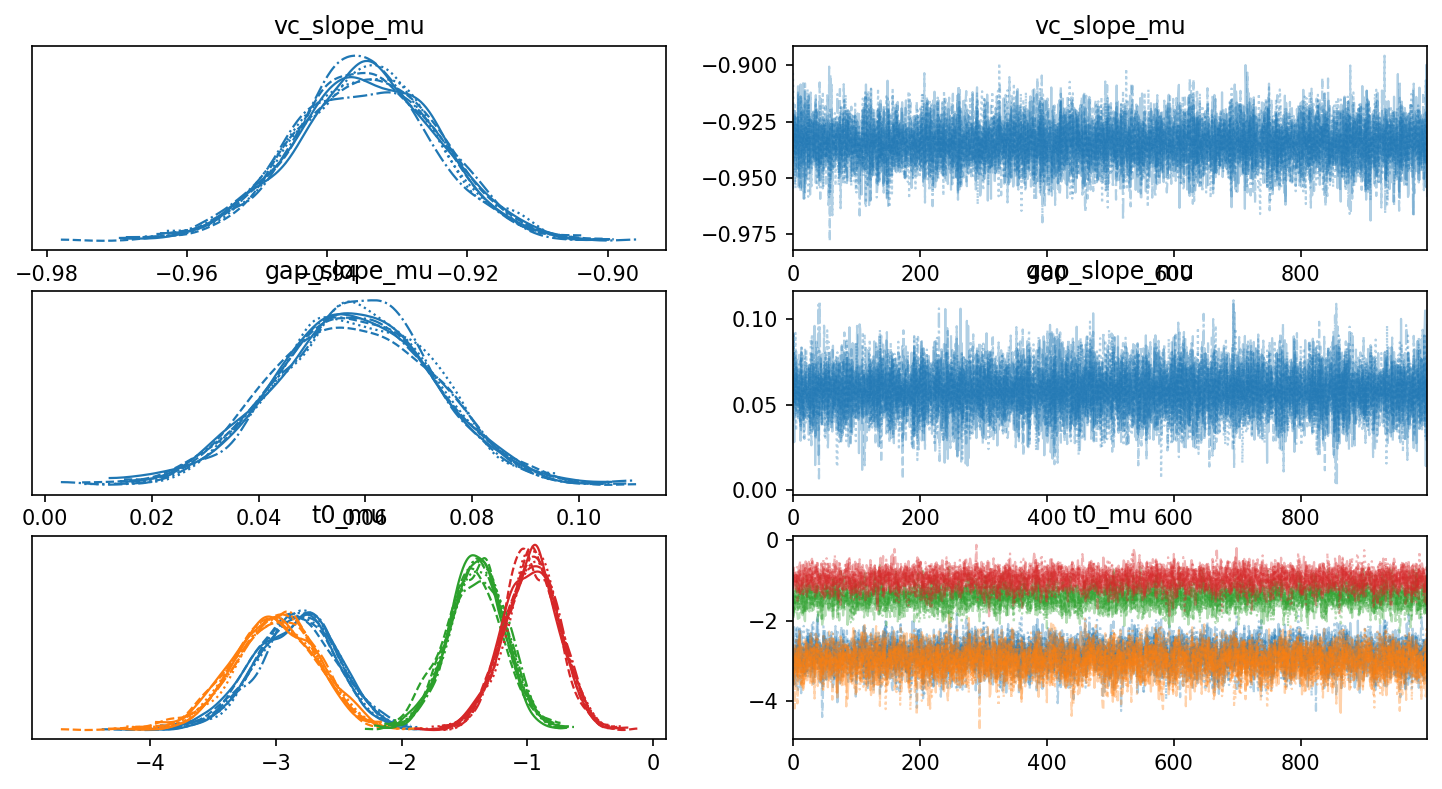
\includegraphics[width=0.9\linewidth,height=\textheight,keepaspectratio]{../../outputs/LBA/lba_trace_plot.png}

}

\caption{\label{fig-lba-trace}MCMC trace plots for key LBA parameters.
Left panels: posterior densities; right panels: sampling chains. Drift
rate slope (ID) and threshold slope (pressure) show unimodal posteriors
and good mixing; non-decision time reflects the four condition-specific
estimates.}

\end{figure}%

\subsection{Adaptive System Manipulation
Check}\label{adaptive-system-manipulation-check}

Hand width inflation did not activate in this dataset. Across all
trials, \texttt{width\_scale\_factor} remained 1.0 (0 trials with
scaling). The PolicyEngine emitted \texttt{inflate\_width} actions in
some sessions, but the UI integration did not apply them to rendered
targets. Consequently, hand UI-mode effects cannot be interpreted as
adaptation effectiveness; only gaze declutter was evaluable. Full
diagnostic analysis is available in the project repository.

\section{References}\label{references}

\phantomsection\label{refs}
\begin{CSLReferences}{1}{0}
\bibitem[\citeproctext]{ref-bahill1979}
Bahill, A. T., \& Stark, L. (1979). The trajectories of saccadic eye
movements. \emph{Scientific American}, \emph{240}(1), 108--117.

\bibitem[\citeproctext]{ref-bridgeman1975}
Bridgeman, B., Hendry, D., \& Stark, L. (1975). Failure to detect
displacement of the visual world during saccadic eye movements.
\emph{Vision Research}, \emph{15}(6), 719--722.

\bibitem[\citeproctext]{ref-brown2008}
Brown, S. D., \& Heathcote, A. (2008). The linear ballistic accumulator
model of simple choice and reaction time. \emph{Cognitive Psychology},
\emph{57}(3), 153--178.

\bibitem[\citeproctext]{ref-dey2001}
Dey, A. K. (2001). Understanding and using context. \emph{Personal and
Ubiquitous Computing}, \emph{5}(1), 4--7.
\url{https://doi.org/10.1007/s007790170019}

\bibitem[\citeproctext]{ref-grossman2005bubble}
Grossman, T., \& Balakrishnan, R. (2005). The bubble cursor: Enhancing
target acquisition by dynamic resizing of the cursor's activation area.
\emph{Proceedings of the SIGCHI Conference on Human Factors in Computing
Systems}, 281--290.

\bibitem[\citeproctext]{ref-herling2010}
Herling, J., \& Broll, W. (2010). Advanced self-contained object removal
for realizing real-time diminished reality in unconstrained
environments. \emph{2010 IEEE International Symposium on Mixed and
Augmented Reality}, 207--212.

\bibitem[\citeproctext]{ref-iso2000}
ISO 9241-9: Ergonomic Requirements for Office Work with Visual Display
Terminals (VDTs) --- Part 9: Requirements for Non-Keyboard Input Devices
(2000).

\bibitem[\citeproctext]{ref-jacob1990eye}
Jacob, R. J. (1990). What you look at is what you get: Eye
movement-based interaction techniques. \emph{Proceedings of the SIGCHI
Conference on Human Factors in Computing Systems}, 11--18.

\bibitem[\citeproctext]{ref-kim2025pinchcatcher}
Kim, J., Park, S., Zhou, Q., Gonzalez-Franco, M., Lee, J., \& Pfeuffer,
K. (2025). PinchCatcher: Enabling multi-selection for gaze+pinch.
\emph{Proceedings of the CHI Conference on Human Factors in Computing
Systems}.

\bibitem[\citeproctext]{ref-lerche2017}
Lerche, V., Voss, A., \& Nagler, M. (2017). How many trials are required
for parameter estimation in diffusion modeling? A comparison of
different optimization criteria. \emph{Behavior Research Methods},
\emph{49}, 513--537.

\bibitem[\citeproctext]{ref-mackenzie1992fitts}
MacKenzie, I. S. (1992). Fitts' law as a research and design tool in
human-computer interaction. \emph{Human-Computer Interaction},
\emph{7}(1), 91--139.

\bibitem[\citeproctext]{ref-majaranta2006}
Majaranta, P., MacKenzie, I. S., Aula, A., \& Räihä, K.-J. (2006).
Effects of feedback and dwell time on eye typing speed and accuracy.
\emph{Universal Access in the Information Society}, \emph{5}(2),
199--214.

\bibitem[\citeproctext]{ref-martinezconde2004}
Martinez-Conde, S., Macknik, S. L., \& Hubel, D. H. (2004). The role of
fixational eye movements in visual perception. \emph{Nature Reviews
Neuroscience}, \emph{5}(3), 229--240.

\bibitem[\citeproctext]{ref-mcguffin2005}
McGuffin, M., \& Balakrishnan, R. (2005). Fitts' law and expanding
targets: Experimental studies and designs for user interfaces. \emph{ACM
Transactions on Computer-Human Interaction (TOCHI)}, \emph{12}(4),
388--422.

\bibitem[\citeproctext]{ref-meyer1988}
Meyer, D. E., Abrams, R. A., Kornblum, S., Wright, C. E., \& Smith, J.
E. K. (1988). Optimality in human motor performance: Ideal control of
rapid aimed movements. \emph{Psychological Review}, \emph{95}(3),
340--370.

\bibitem[\citeproctext]{ref-patney2016}
Patney, A., Salvi, M., Kim, J., Kaplanyan, A., Wyman, C., Benty, N.,
Luebke, D., \& Lefohn, A. (2016). Towards foveated rendering for
gaze-tracked virtual reality. \emph{ACM Transactions on Graphics (TOG)},
\emph{35}(6), 1--12.

\bibitem[\citeproctext]{ref-pfeuffer2024gaze}
Pfeuffer, K., Gellersen, H., \& Gonzalez-Franco, M. (2024). Design
principles and challenges for gaze + pinch interaction in XR. \emph{IEEE
Computer Graphics and Applications}, \emph{44}(3), 74--81.
\url{https://doi.org/10.1109/MCG.2024.3382961}

\bibitem[\citeproctext]{ref-pfeuffer2017gaze}
Pfeuffer, K., Mayer, B., Mardanbegi, D., \& Gellersen, H. (2017). Gaze+
pinch interaction in virtual reality. \emph{Proceedings of the 5th
Symposium on Spatial User Interaction}, 99--108.

\bibitem[\citeproctext]{ref-reason1990}
Reason, J. (1990). \emph{Human error}. Cambridge University Press.

\bibitem[\citeproctext]{ref-saunders2014}
Saunders, D. R., \& Woods, R. L. (2014). Direct measurement of the
system latency of gaze-contingent displays. \emph{Behavior Research
Methods}, \emph{46}(2), 439--447.

\bibitem[\citeproctext]{ref-soukoreff2004towards}
Soukoreff, R. W., \& MacKenzie, I. S. (2004). Towards a standard for
pointing device evaluation, perspectives on 27 years of fitts' law
research in HCI. \emph{International Journal of Human-Computer Studies},
\emph{61}(6), 751--789.

\bibitem[\citeproctext]{ref-sweller1988}
Sweller, J. (1988). Cognitive load during problem solving: Effects on
learning. \emph{Cognitive Science}, \emph{12}(2), 257--285.

\bibitem[\citeproctext]{ref-ware1987}
Ware, C., \& Mikaelian, H. H. (1987). An evaluation of an eye tracker as
a device for computer input. \emph{Proceedings of the CHI+GI '87
Conference on Human Factors in Computing Systems and Graphics
Interface}, 183--188.

\bibitem[\citeproctext]{ref-williams1949experimental}
Williams, E. J. (1949). Experimental designs balanced for the estimation
of residual effects of treatments. \emph{Australian Journal of
Chemistry}, \emph{2}(2), 149--168.

\end{CSLReferences}




\end{document}
